%!TEX TS-program = xelatex %!TEX encoding = UTF-8 Unicode
\documentclass{zc-thesis}
%\usepackage{draftwatermark}          %use these two lines for draft
%\SetWatermarkText{DRAFT}\SetWatermarkScale{1}\SetWatermarkColor[rgb]{0.9,0.5,0.5}

\begin{document}
\hypersetup{pdfauthor={Zhang, Chao},    pdfcopyright={Copyright (C) 2017 by Zhang, Chao.
    Licensed under CC-BY-SA 4.0. Some rights reserved.},
    pdflicenseurl={https://creativecommons.org/licenses/by-sa/4.0/}} 
\title{Probing Nanomaterial Properties in a High-Resolution Transmission Electron Microscope}

\author{Chao Zhang}
\advisor{Dmitri Golberg}

\degree{Doctor of Philosophy}
\field{Materials Science and Engineering}
\degreeyear{2017}
\degreemonth{February}

\department{Pure and Applied Sciences}
\university{University of Tsukuba}
\universitycity{Tsukuba}
\universitystate{Ibaraki}
\maketitle 
\copyrightpage\dedicationpage\abstractpage\acknowledgments\tableofcontents
\onehalfspacing\listoffigures\listoftables \afterpage{\null\newpage}
\pagestyle{fancy}\fancyhf{}
\fancyhead[RE]{\scriptsize \nouppercase \rightmark}
\fancyhead[LO]{\scriptsize \nouppercase \leftmark}
\fancyfoot[LE]{{\LARGE \bf \thepage} \hspace{15pt} 
.....................................................................................................................................................................}
\fancyfoot[RO]{
..................................................................................................................................................................... \hspace{15pt} {\LARGE \bf \thepage}}

\setlength{\textfloatsep}{10pt plus 1.0pt minus 2.0pt}  %floats length
\setlength{\floatsep}{10.0pt plus 1.0pt minus 2.0pt}
\setlength{\intextsep}{10.0pt plus 1.0pt minus 2.0pt}

%update: Jan 13 fixed gramma according to prof notes
%update: Jan 09-11 prof check
%update: Dec 20 finish wrting
%update: Nov 09 Prof checked some of the texts

%\begin{savequote}[75mm] 
%There's plenty of room at the bottom.
%\qauthor{Richard Feynman} 
%\end{savequote}

\chapter{Introduction}

\newthought{The} advancement of material science and technology has led to the discovery and utilization of nanoscale materials. Many of these new materials possess extraordinary chemical, electrical, optical or mechanical properties. However, as human beings, who are millions or billions times larger than nanomaterials, we are not perfectly scaled to reach them directly. As Feynman said, there is plenty of room at the bottom, but it also means that plenty of efforts are expected toward researching. 

\begin{figure} 
\centering
\includegraphics[width=400pt]{figures/figure1_factors}
\caption[Factors and applications]{Special factors of nanomaterials contributing to various applications. 
\label{fig:1_factor}}
\end{figure}

%nanoscale--nanomaterials--to see--to manipulate
\section{Probing of nanomaterials}
%what is nanomater...why nanomater...
Generally, nanomaterials are materials in which a single unit is sized from one nanometer to a few hundred nanometers. The scale difference between these materials and human body is more than a million. Besides scale difference, nanostructures usually possess special properties as compared with bulk materials due to chemical composition difference, surface to volume ratio and quantum confinements. The confined structures of the same chemical type and composition might present very different properties. An easy way to understand a value of the nanomaterial is to consider carbon materials. We know diamond and graphite are allotropes of carbon which possess different bonding and thereby amazingly distinct physical and chemical characteristics. This is also true for a fullerene, a carbon nanotube and graphene. Even the number of walls in a carbon nanotube would significantly affect its properties. \cite{rodunerwhynano2006} Therefore, what makes nanostuctures distinctive is not only their size, but also their unique compositions, surface and quantum confinement effects. 

\renewcommand{\thefootnote}{\fnsymbol{footnote}}

As shown in Figure \ref{fig:1_factor}, all effects contribute to the particular functionality of a nanomaterial, such as superior mechanical strength and rigidity, ultrahigh electrical mobility, abundant chemical active sites, ect. Mechanical superiority is important for mechanical applications, such as flexible electronics and devices in Nano Electro-Mechanical Systems (NEMS). Electrical superiority of nanomaterials with various electronic band structures could be applied in electrical diodes, transistors, laser diodes (LDs), light-emitting diodes (LEDs), and in transparent or flexible electronics and optoelectronics. Chemical superiority of nanomaterials make them desirable for high efficiency catalysis and portable energy storage devices with high energy density. 

%limitations to study nanomater...

\begin{figure} 
\centering
\includegraphics[width=\textwidth]{figures/figure1_scale_problem.pdf}
\caption[Scale problem]{How human beings gain access to lower scales, to see and to manipulate.\footnotemark[1]
\label{fig:1_scale}}
\end{figure}

However, it is not straightforward to access the properties of these nanomaterials and prepare them for real applications. Unfortunately this is due to the above-mentioned issue - small scale. We understand that the observation, reach and built of an object which is $10^6$ to $10^9$ (in one dimension) smaller then any real world macro-object, for example the {\em Great Wall of China} ($21,196 km$), is challenging. Similarly, as compared with human beings' hands, of a size is about $20 cm$, nanoscaled objects are usually million times smaller. Hence, even the nanoscale building blocks are superior in many respects in theory, we are not able to utilize them easily. As shown in Figure \ref{fig:1_scale} \footnote{Without specification, all clip art materials (elephant, ant, microscope, tweezers, etc.) in figures of the dissertation are adapted from Internet which are {\em free to use without permission}.}, we are able to reach smaller scales using tweezers and optical microscopes, but it is very challenging to reach nanoscale objects. 

%introduce to microscopy and probing tech. 
The way human beings make use of fire, tools,  light and electrons is perhaps what sets our modern live standards above of other species. By understanding and utilizing photons, electrons and atomic forces, microscopy allows us to view sub-millimeter objects that cannot be observed with a naked eye. Thanks to the advancement of tools - microscopy and piezoelectric materials - we can now access to nanomaterials by high precision probing technique under direct high-resolution observations. By applying electrical field to a piece of piezoelectric material, the latter precisely changes its shape in function of the applied electric field. Therefore, we may control the mechanical movements by electrical biases and confirm the location of an object and the probe using microscopy. 

\begin{figure}  
\centering
\includegraphics[width=320pt]{figures/figure1_to_study_nanomater.pdf}
\caption[Study of nanomaterials]{{\em In situ} TEM serves as a way to study nanomaterials.
\label{fig:1tsn}}
\end{figure}
%what is in situ TEM

\section{Seeing is believing: Transmission Electron Microscopy}
In the past century, development of particle physics made a way for new microscopies, such as Scanning Probe Microscopy (SPM, including Atomic Force Microscopy and Scanning Tunneling Microscopy), Scanning Electron Microscopy (SEM), and Transmission Electron Microscopy (TEM). Among all microscopies TEM, has the best ultimate spatial resolution; this allows one to reach atomic resolution and to simultaneously get full crystallography information. TEM provides deep and direct information from a thin sample through the transmission and diffraction of electrons. 

When researchers are not satisfied with only seeing of a material in statics, dynamics may be introduced to the sample. \emph{In situ} TEM is the newest advanced technique which gives access to the sample dynamics via observation, manipulation and various tests.\\
Particularly, by adapting the microscope or using a special specimen holder, it is possible to make deliberate attempts to modify materials during high-resolution characterizations. It allows for the observation of dynamic properties of a material under special circumstances.\cite{banhart2008situ}\\

\begin{figure}  
\centering
\includegraphics[width=300pt]{figures/figure1_TEM_As_Microscopy.pdf}
\caption[\emph{In situ} TEM as a microscopy branch]{Relationships between probing \emph{in situ} TEM and other microscopies.
\label{fig:1tam}}
\end{figure}

For instance, a heating holder would provide the desired high temperature to trace (by a fast CCD video camera) and thereby reveal chemical transformations within a sample. By contrast, without \emph{in situ} heating, one is  only able to see the initial and final states of the reaction; in this way the regarded mechanism is usually inferred based on a few indirect clues, such as X-ray Diffraction (XRD), X-ray photoelectron spectroscopy (XPS), Energy Dispersive X-ray Spectrometry (EDS), Photoluminescence (PL) and indirect TEM characterizations before and after the dynamic tests. As illustrated in Figure \ref{fig:1tsn}, \emph{in situ} TEM is very important and irreplaceable approach to study nanomaterials. \\

Various specimen holders make it possible to introduce heating, cooling, electrical bias, mechanical force, gas, liquid, magnetic field, light etc. to the sample under various conditions. As illustrated in Figure \ref{fig:1tam}, probing \emph{in situ} TEM is one small domain of microscopy as a whole. This Dissertation is mainly focused on probing of nanomaterials via \emph{in situ} TEM. 

%probing in situ TEM
\section{Untouchable scale: Probing techniques for nanomaterials}

Experiments performed by \textit{in situ} probing microscopy are carried out based on piezoelectric effect and microscopy. \\

\begin{figure}  
\centering
\includegraphics[width=250pt]{figures/figure1_piezo.pdf}
\caption[Probing by piezoelectronics]{Schematic illustration of how piezoelectric works for precised nanomanipulations.
\label{fig:1piezo}}
\end{figure}

Piezoelectricity is a phenomenon where electricity is directly related to the pressure applied to the material. In a piezoelectric actuator, special driving signals are applied to a piezoelectric tube in certain directions, and thereby the piezoelectric tube would respond while changing shape accordingly.\cite{okada2004piezoelectric,vishnevsky1977piezoelectric} As shown in Figure \ref{fig:1piezo}, when the base of the tube is fixed, transverse and axial movements of the tube tip would be expressed approximately by the following equations:
$$\begin{bmatrix}\Delta x\\ \Delta y\end{bmatrix}= \frac{2\sqrt{2}d_{31}}{\pi Dh}L^2\begin{bmatrix}U_{+x}-U_{-x}\\U_{+y}-U_{-y} \end{bmatrix},$$
$$\Delta L= \frac{d_{31}L}{h}V$$
, where $\Delta x$, $\Delta y$ and $\Delta L$ are deflection in $x$, $y$ and axial direction. $U_{+x}-U_{-x}$, $U_{+y}-U_{-y}$ are driving voltages applied to the opposite sides of the tube (therefore in total four electrodes, in addition to the base ground electrode).$V$ is voltage applied to all four quadrants. $L$, $D$ and $h$ is the length, diameter and thickness of the tube. The transverse piezoelectric coefficient $d_{31}$  is very small (about $-10^{-10} \mathrm{m/V}$), and, hence, the movement can be controlled precisely by biasing. 

With a help of a piezoelectric actuator, we can handle an ultrasharp probe to touch the nanoscale sample with the nanometer precision. 
\\
Now we have two effective ways to see and touch a nanostructure -- {\em in situ} TEM and piezo-motor-driven probing. 


\section{Optoelectronic and flexible electronic applications of nanomaterials}
%light to replace electrons
We are currently fully enjoying the benefits of well developed microelectronics and nanoelectronics. However, people are trying to improve the speed of information transmission by means of light. As compared with electrons in the metal (copper or even gold) conductors, photons in the optical system possess much higher capacity of information. The society benefits a lot from the optical fiber information technology. For instance, it was quite difficult and expensive to perform high-definition video streaming \textit{via} Internet 20 years ago when we were using copper wires to transmit electrical information. 
%silicon is not best for optoelectronics
The silicon-based electronics is efficient and is mainly based on the two materials: silicon and copper (or other conductors such as gold). The manufacturing is sophisticated and requires etching silicon chips and applying a mask for electrode coating. Silicon is absolutely perfect semiconducting material. By doping techniques and smart designs, billions of transistors could work at a high speed within a nail-sized chip. The problem is (for optoelectronic applications) that the band-gap diversity is required. Therefore silicon, as a perfect semiconductor for electronics, could not realize fully functioning optoelectronics. \\ 
%silicon is not best for flexible electronics
Besides, flexible electronics attracts a great deal of attention. In the last few years, we experienced an explosion of flexible optoelectronic applications in flat-panel displays, lighting, sensing, and energy cells. For instance, organic light-emitting diodes (OLED) and flexible lithium-ion batteries are developed as a next-generation technology for wearable electronics, bendable smart-phones, foldable displays, etc. However, to make silicon wafers flexible is never an easy task. Therefore, people believe that the bottom-up technology would be able to architect nanoscale building blocks on a flexible substrate for future flexible electronics and optoelectroncs. \\

\begin{figure}  
\centering
\includegraphics[width=340pt]{figures/figure1_silicon.pdf}
\caption[Future of optoelectronics and flexible electronics]{Silicon's two short-comings for flexible devices and optoelectronics could be backed-up by bottom-up approach using nanomaterials in future integrations.
\label{fig:1si}}
\end{figure}

%So nanomater is good for optoelectronics and flexible applications
Therefore, for optoelectronic and flexible electronic applications, the usage of conventional silicon industries is challenging, as shown in Figure \ref{fig:1si}. Silicon  is an ideal material to meet all requirements within a field effect transistor. The silicon based devices rely on controlling carriers realized \textit{via} structural design and doping. In recent years, silicon-based optoelectronics is growing steadily but not exponentially, as expected by Moore's Law. \cite{Waldrop2016} 
The semiconductor industries produce devices mainly by the top-down strategy. A top-down approach is a smart way to apply desired patterns to the device engineering, which came in effect since 1970s, when human beings were not so experienced to manipulate nanostructures. However, these days a bottom-up approach is emerging and shows a high promise in constructing systems by piecing building blocks together. It is true that some nanomaterials show superior properties for electronics, but it appears that during the last decade, many efforts from various research groups have been unable to establish bottom-up technology as a real market value. \\
It is expected that in the future high quality nanomaterial building blocks could be well handled for device integrating by the automated mass production. The integrated LDs, LEDs and photodetectors could be manufactured using nanowires, nanosheets and even quantum dots to realize fully functioning optoelectronic chips. The current obstacle is to get more knowledge of the building block materials. How does the electrical signal from nanowires or nanosheets behaves under strain and light illumination, what is the photocurrent spectroscopy of the material - such questions are not well studied. Consequently, it is strongly required that we find the answers to these questions in order to provide clues for future flexible electronics and optoelectronics. 

\section{Energy storage applications of nanomaterials}
%energy is important
Electrical energy storage will be far more important nowadays than it was when we had abundant petroleum resources, and when we didn't have smart (smart also means energy consuming) electronics. From powering portable electrical devices (cell phones, tablets, laptops), implantable medical applications (pacemaker), to machines (hybrid electric vehicles), the humans' desire for clean, safe, fast and efficient energy storage is becoming more and more  significant. \\
%ion-batter is important
Among all energy storage applications, lithium ion-batteries (LIBs) are the most needed devices due to their high energy density, which is the key factor for portable electronics and automobiles. In LIBs, lithium ions move from the anode to cathode during discharge, and from cathode to anode during charging. The materials for the anodes and cathodes can dramatically affect the few key aspects of the battery’s performance, including stability and capacity. High capacity materials are eagerly demanded in order to address the needs for better energy density, cycle life and charge lifespan, among other issues faced by Li-ion batteries. 
%Nanomater for ion-battery
However, conventional materials, although being  well developed,  still cannot catch up with the growing demands of battery capacity. Li-ion batteries have struggled with numerous issues, such as poor cycle life, rising internal resistance with cycling and aging, safety concerns (especially when overheated or charging problem), and growing applications demanding higher capacity. \\
A lot of researches have confirmed that nanomaterials are particularly promising to solve these problems. The advantages are as follows\cite{Bruce2008,qifengzhang2013csr}: \\
\begin{itemize}
	\item[a] Many nanomaterials enable electrode reactions to become reversible while they are not reversible for bulk materials; 
	\item[b] The reduced size significantly increases the rate of energy transformation between electricity to chemical energy (such as lithiation and delithiation process) due to the short diffusion lengths; 
	\item[c] Electron conductivity can also be improved in nanomaterials; 
	\item[d] High surface to volume ratio provides high contact area between electrodes and electrolyte; 
	\item[e] Chemical potentials of ions and electrons can be different at the nanometer scale, and, therefore, electrode potential can be modified. 
\end{itemize}

\begin{figure}  
\centering
\includegraphics[width=340pt]{figures/figure1_lib.pdf}
\caption[Future of secondary ion batteries]{\textcolor{red}{Current secondary batteries are mostly based on Lithium and graphite. However, to gain higher energy density while at the same time to use cheaper/abundant elements, nanomaterials might be the key. }
\label{fig:1lib}}
\end{figure}

%silicon for ion battery anode
 Graphite has widely been used as an anode of choice for commercial products, since the first generation of Li-ion chemistry studies appears. Due to strong needs of high capacity, in recent years, researchers have been interested in developing silicon anode materials for high capacity lithium-ion batteries. Among all investigated anode materials, silicon has one of the best  theoretical capacities of $3590 \mathrm{mAh/g}$ (about 10 times higher than carbon) based on the fully alloyed form of \ce{Li15Si4} at room temperature (at high temperature \ce{Li15Si4} can be obtained, giving a capacity of $4200 \mathrm{mAh g−1}$, placing it on top of all other anode materials. In addition, Si anodes show moderate working potential at $0.5$ V, which is higher than graphite anodes at $0.05 $ V. This means that silicon is suitable to solve the safety problem of lithium deposition upon cell overcharge as well as avert the energy penalty of battery cells assembled with the \ce{Li4Ti5O12} anodes.\\
 However, the insertion/extraction of lithium ions result in significant volume change - about 370\% - which leads to structural pulverization and electrical disconnection between anode materials and current collector, and finally the battery loses most of its functions. Some recent designs of LIBs using silicon materials as anodes allows the battery to maintain its initial anode structure and hence to reach high capacity while, at the same time, good stability. 

 Cui et al. designed high performance anode structure using Si nanowires, which were able to accommodate large strain caused by lithium ion insertion and extraction.\cite{Cui2009} 
 Deng et al. reported a tubular configuration made from rolled-up C/Si/C layered nanomembranes which performs with a highly reversible capacity at approximately 2000 mAh /g (50 mA/g), and has approximately 100\% capacity retention (500 mA/g) after 300 cycles.\cite{Deng2013}
 Cui et al. also designed core-shell structures for Si-based LIBs. They proposed a hierarchically structured Si anode which was inspired by the structure of a pomegranate. Si nanoparticles became encapsulated by conductive carbon coatings. This leaves just enough space for the expansion and contraction during lithiation and delithiation cycles. \cite{Liu2014d}
   
\begin{figure}  
\centering
\includegraphics[width=\textwidth]{figures/figure1_silibdesign}
\caption[Designs for large volume expansion anode materials]{Designs for large volume expansion anode materials in batteries. Red correspond to material with large volume expansion/shrinking during cycling, while material in blue color is the confinement material with low volume expansion rate and good mechanical strength. 
\label{fig:1silibdesign}}
\end{figure}
 
Therefore, by designing the microscopic structures, one is able to utilize the high capacity material under structural and mechanical restrictions, as illustrated in Figure \ref{fig:1silibdesign}. Also, many other attempts of combining silicon with carbon materials,  polymers,  metals, were summarized by Liang et al.\cite{Liang2014} 
 
%Na-ion batteries
It is predicted that lithium would be the next energy resource which substitutes for petroleum, which will die out.\cite{Jaskula2016} According to the distribution of lithium on Earth\cite{Jaskula2011}, Chile could be the next Saudi Arabia it terms of richness of resources. This problem is more essential for many countries with very limited lithium reserves, such as Japan. \\
In order to explore the next generation of secondary batteries, which are called post-lithium ion secondary batteries, many investigations
show that the most promising candidate is the sodium-ion battery (SIB). SIBs use sodium instead of lithium as the charge carrier, and use iron, manganese and other transition metals to replace cobalt for redox reactions. SIBs are expected to be mass produced in the nearest future due to their minor environmental impacts and low cost.

\begin{table}[ht]
\centering % used for centering table
\begin{tabular}{|l|c|c|} % left, centered columns (3 columns)
\hline %inserts double horizontal lines
 & LIB & SIB\\ [0.5ex] % inserts table heading
\hline % inserts single horizontal line
Theoretical capacity & 3,829 mAh/g & 1,165 mAh/g \\[1.5ex] % inserting body of the table
Cost (carbonate) & 5,000 USD/t & 150 USD/t \\[1.5ex]% [1.5ex] adds vertical space
Reserves & 23,000 ppm & 20 ppm \\[1.5ex]
Potential & –3.045 V & –2.714 V \\[1.5ex]
Ionic radii & 79.3 pm & 100.9 pm \\[1.5ex]
\hline %inserts single line
\end{tabular}
\caption{Comparison of LIB with SIB.} % title of Table
\label{table1.1} % is used to refer this table in the text
\end{table}

As shown in Table \ref{table1.1}, although sodium possesses a higher normal electrode potential of ~0.3 V, larger effective radius than lithium (in volume ratio 2.05), and smaller theoretical capacity, the cost and environmental benefits are still very attractive for applications which do not require very high capacity. Actually, it is hard for graphite, which is commercially used as an anode material for LIBs, to store and release sodium ions both theoretically and in practice because of the size of sodium ion is large. \\
However, it was discovered in 2000 that hard carbon having disordered structures could electrochemically store and release sodium ions.\cite{Stevens2000} Several years ago, a work was done on developing and making practical sodium ion batteries, and since recently researchers have been investigating on many anode active materials for sodium ions. It is worth noting that well-established guidelines and experiences acquired for LIBs electrode active materials are not applicable for SIBs.\cite{Lang2010,Armand2008,KUZE2013}

Consequently, the two important research areas of secondary batteries are: finding better anode active materials with higher capacities, and looking for other elements for ion batteries, as illustrated in Figure \ref{fig:1lib}. To apply these elements in secondary batteries, nanomaterials, or nanoscaled designs play very important roles. They enable reactions which may overcome huge volume expansion, to decrease diffusion lengths; while bulk materials are not capable to reach the highest capacity either for LIBs or for special ion-batteries at the moment. 

\section{Motivation of my PhD research}
As stated above, {\em in situ} studies on nanomaterials toward optoelectronics, electronics and ion batteries are required by the Society. My motivation is to take the challenge and to analyze the dynamics of the building blocks, as well as heterostructures, and to provide decent knowledge for advanced applications. 
Therefore, I explored some experimental methods and engineering details, including {\em in situ} TEM setups and the working mechanisms. \\
Then I present manipulation possibilities in the frame of the general \textit{nanoarchitectonics} concept and its applications for nanoengineering. The experiments have been performed on the {\em in situ} TEM-constructed axial nanowire junctions of CdS and p-Si. In addition, detailed electrical probing for energy storage research is discussed. I fabricated an ultra-stable sodium ion battery and analyzed the mechanism of its cycling performance under {\em in situ} TEM probing. Through coupling with {\em in situ} TEM applied mechanical forces, two examples of force-driven optoelectronic phenomena are detailed using the examples of ZnO and CdS. 
%update: Jan 13 add figure 4ways
%update: Jan 09-11 prof check
%update: finish writing Dec 30
%note: image 4waysprobe is not here

%\begin{savequote}[75mm] 
%We become what we behold. We shape our tools, and thereafter our tools shape us.
%\qauthor{Marshall McLuhan} 
%\end{savequote}

\chapter{Engineering of Probing Techniques inside TEM}

\newthought{We are not satisfied with the limited possibilities provided by TEM}, and we are eager to introduce more variables to the system because that is how we see dynamics in the real applications.
In the following subsections, I will firstly introduce how we cooperate chemicals, light, mechanical manipulations and electrical interactions within the microscopic experiment. 
Especially for the new optical fiber compatible TEM, where all the four factors could be merged, the inside and outside parts of the \emph{in situ} microscopic setup are described in detail. 
Finally I will take a look at the what the system can do and its short-comings. 

%before us, stm tem holder
\section{Introducing chemicals, electricity, strain into the microsocpe}

As I discussed in Chapter 1, \emph{in situ} microscopy does introduce parameters such as heat, cooling, gas, liquid, etc. to the system, but now I focus on how we delicately introduce these variables into the  microscope. In most cases, {\em in situ} microscopic experiments are performed by means of specially designed TEM holders, such as heating holder equipped with heating electrical wire or MEMS microheater. At the same time, some researchers made adaptions to the  microscope to introduce other variables. In my Ph.D. research, in addition to the electron beam, four more variables are introduced: chemicals (solid), mechanical probing, electrical contacting and optical access. \\

For electrical biasing, many TEM holders are commercially available. Such holders provide a combination of TEM and Scanning Tunneling Microscopy(STM) techniques, which are employed simultaneously within one instrument. TEM characterization, STM imaging, introducing chemicals and electrical measurements- all become possible. The STM probe scanner has a very wide range of motions, from picometers to millimeters, which are employed either for a coarse adjustment of the sample orientation, or for a precise probe positioning. \\

Electrical contacts with nanoscaled interfaces can be realized under precise positioning of the movable probe to the desired spot, enabling simultaneous investigation of the specimen’s structural and electronic  properties with the optional strain or chemical transitions.\\

If the electrical biasing is realized through piezo probing, we can also utilize the probe for introducing chemical (solid on probe) and mechanical strain (without force value measurement\footnote{Introducing atomic force microscopy into TEM holder for mechanical measurements is another important {\em in situ} method without electrical biasing functions.}). \\

I briefly discussed the ways to input chemical, electrical biasing and mechanical factors in TEM. However, introducing  the other variable - light - to the system is challenging. Therefore I will discuss this part separately, which would be a very good reference for future research, in the next section. 

\section{Introducing light into the microscope}
\subsection{Previously}
Introducing the other factor - light - to the system, while at the same time maintaining the impact from other factors, is very tricky. Some researchers and companies tried to introduce light without probing. This means that no introduction of chemical changes, electricity and mechanics was achieved. We may first investigate how they introduce/collect light to/from the microscope. 
Table \ref{table2.1} compares the two possible ways to implement light into the system. 

\begin{table}[ht]
\centering 
\begin{tabular}{|c|c|} 
\hline 
by adaption to the microscope & by using special holder \\ [0.5ex] 
\hline 
light plane different from specimen & on same plane with specimen \\[1.5ex] 
require take off detector/aperture & a specially designed holder \\[1.5ex]
optics can be realized by lens on bench & only optical fiber\footnote{For the moment only optical fiber, but it is possible to have lens system inside the holder, please read Chapter 7 for more information.} \\[1.5ex]
complicated, high power, high cost & no adaption to TEM\\[1.5ex]
\hline
\end{tabular}
\caption{Two main ways to implement light into a TEM} 
\label{table2.1} 
\end{table}

As shown in the Table, by replacing an aperture or making a window for optical path the light path becomes tilted. The light goes through the microscope body at the different level from the specimen plane. In some cases, it is possible to replace a detector or an aperture by desired modules to provide more variables. As shown in Figure \ref{fig:2_1} under a certain angle, the light can reach the specimen. The system could be very complicated if the optics is realized through lens system on optical bench including light sources, lens system and options such as CCD camera, chopper and monochromator. The system can be very powerful if the optical system on table is well designed and precisely assembled. However, the pressure of time and high cost are expected to be very significant. \\

\begin{figure}  
\centering
\includegraphics[width=320pt]{figures/figure2_1}
\caption[Putting light into TEM.]{How light is compatible to TEM.
\label{fig:2_1}}
\end{figure}

For a special optical holder, one way is to protrude an optical fiber through the holder, as shown in Figure \ref{fig:2_1}, the light will be shinning on the specimen at about 90 degrees to the direction of the electron beam. In most cases, the microscope is owned by many users for various applications, and therefore the approach of using special optical holder is more practical - it's quite unpractical to drill a hole in the microscope column and to install an optical bench on the microscope (given the fact that not every user will be happy with such operations). 

A few groups have tried to deliver light into TEM. \\

Muto et al. (Kyushu University) managed to install an optical fiber through a 2 mm hole at an angle of 45 degrees.\cite{Tanabe2002,Furumoto2013} They manufactured the prototype of TEM-CL system with the light collecting parts integrated on the holder, but no parabolic reflector was needed within the pole piece. The system is able to take cathodoluminescence(CL), X-ray emission spectroscopy and Electron Energy Loss Spectroscopy(EELS) at the same time, even under large angle sample tilts. The main disadvantage of the holder was a significant background level from the thermal glow of the electron gun and the CL signal from the optical fiber. Later, Muto et al. and staff from {\em Nanofactory Instruments} developed a prototype optical holder implemented with an optical fiber through the holder, on the side of a specimen. The reflectors and optical fiber are placed away from the TEM optical axis. The light-collecting solid angle is approximately 1.3 strad, approximately 100 times larger than that of their first generation prototype. The sample is mounted at the end of the metal wire, which  position can be controlled to the focal point of the mirror by the piezo-driven manipulator. In years of 2012-2013, a few groups, including us, secured the optical holder (beta version) from {\em Nanofactory Instruments}. \\

One of the groups is in Brookhaven National Laboratory. Yimei Zhu et al. obtained the prototype optical holder from {\em Nanofactory} which allows for two optical fibers and several delicate mirrors to locate the light beam to the specimen. 
The multimodal optical nanoprobe allows scientists to perform standard experiments natural for TEM in addition to those involving optical excitation and measurements on the sample, including electrical measurements, STM and combinations of those. They emphasized the ability to simultaneously measure optical and electrical properties of the sample at the nanoscale.\cite{Zhu2012Multimodal}  The operations introduced are very similar to our case, but their serious problems were related to the calibration of light spot location, which is realized by the adjustment of the tiny mirror screws; also, they were not able to confirm the location of light spot. Therefore the system was not that practical. \\

Minor et al. have implemented a {\em in situ} TEM monitoring technique to observe the crystallization of a-Si during high power pulsed laser irradiation by directly coupling laser into a TEM through a fiber-optics probe. By realizing a near-field scanning optical microscopy (NSOM) fiber probe scheme, this technique opens up a wide variety of new characterization possibilities.\cite{Xiang2012}

Kociak et al. of the Université Paris-Sud \cite{Zagonel2011} developed a STEM-CL system on Nion microscope which also uses an optical fiber as a light guide from the microscope column to the CCD camera outside the microscope. The light is collected by a specially designed mirror system of which the focus point is on the specimen. This CL-STEM imaging can be applied to obtaining luminescence spectra and imaging the structure simultaneously.\cite{Nagarajan2016Simultaneous}

In another group, Miller in Prof. Crozier's group in Arizona State University replaced the EDS detector (first version) or objective aperture (second version on FEI Titan microscope) with an optical fiber to shine a light onto chemicals to observe dynamics of photochemical reactions.\cite{Miller2012} But the problem was that they had not been sure about the location of the light spot, because they could not observe it.

To conclude, by introducing light into TEM, these days the researchers are capable to observe dynamics of photochemical processes or thermo-effects, and to simultaneously obtain high resolution CL with EELS and Dark field imaging. As summarized in Table \ref{table2.2}, almost all groups used optical fibers for introducing light rather than lens system on bench, whereas most groups do not offer probing contacts capabilities. In my case (NIMS in Table), I would like to realize all these functions based on the redesigned optical holder. 

\begin{table}[ht]
\centering 
\begin{tabular}{|c|c|c|c|c|} 
\hline 
Institute & fiber & though & Probing contact & practical for\\ [0.5ex] 
\hline 
Nagoya U. & Yes & hole, holder direct & No & CL\\[1.5ex] 
BNL & Yes & holder by sides & Yes & N/A\\[1.5ex]
LBNL & Yes& holder direct & No & NSOM heating\\[1.5ex]
U. Paris-Sud & Yes & holder direct & No & CL-Map, NSOM\\[1.5ex]
ASU & Yes & detector/aperture & No & Photochem.\\[1.5ex]
NIMS & Yes & holder direct & Yes & all above\\
\hline
\end{tabular}
\caption{Compare of the groups who introduced light to TEM} 
\label{table2.2} 
\end{table}

\subsection{Our holder adaption}
To choose between the fiber technology and the breadboard, it is necessary to define the objectives and a budget. 
A honeycomb core breadboard is complex and powerful to customize optical input/output parameters with high precision. 
However, building of an optical system on a honeycomb core breadboard could be costly. 
At least one optical window should be opened on the body of microscope so as to transmit an aligned laser beam into the chamber, and to collect optical signal from the chamber. 
In contrast, by using an optical fiber, a laser light could be easily introduced into the microscope without breaking the TEM body. 
The solution is to make a continuous hole through a special TEM holder so as to insert an optical fiber in it. The former {\em Nanofactory Instruments AB} developed a holder for our Laboratory with a 250 micrometer pipeline. 

In our system, the microscope is not modified at all, and we integrate all the experimental dynamics through the specimen holder. 

The front frame of the special holder was placed into the 4 mm gap of the TEM pole
piece. And with the optical fiber inserted, the light connection between the TEM chamber and the outer space was realized. 

To develop the whole system based on the regarded general idea, the two issue for the setup should be of our prime concern. One issue is the inner TEM side – how to place the samples, how to design the fiber tip, how to operate and apply/test electrical signals on the samples. The other side is the outer TEM side – board development, space for light source and signal processing.  

\begin{figure}  
\centering
\includegraphics[width=320pt, angle=-90]{figures/figure2_4ways}
\caption[Proposed four ways of holder adaption]{Four ways I proposed to introduce probing to optical holder.
\label{fig:4ways}}
\end{figure}

%%%%%%%%%%%%%%%%%%%%%%%%%%%%%%%%%%%%%%%%%%%%%%%%%%%%%%%%%%%%%%%%%%%%%%%%%%%%%
%%%%%%%%%%%%%%%%%%%%%%%%%%%%%%%%%%%%%%%%%%%%%%%%%%%%%%%%%%%%%%%%%%%%%%%%%%%%%%%
\textcolor{red}{
I proposed 4 ways to add electrical access on the piezo-driven optical fiber based on the \textit{Nanofactory} optical holder, as shown in Figure \ref{fig:4ways}. 
The four ways are: \\
\begin{itemize}
	\item[a)] To build separated arms on the frame and place sample across the arms (which can be very difficult) where it can be also illuminated; 
	\item[b)] To drill a hole on original cap, or make a new hat with two holes to install an additional probe; 
	\item[c)] Based on design b), one end of a gold wire can be placed on electrical pad by wire bonding machine, the other end of wire can be manipulated to make contact with the specimen, therefore in total three electrodes applications are possible; 
	\item[d)] To coat conductive metal onto the surface (cross section is not coated) of optical fiber (which is marked by yellow), the coating conducts the end (edge) of fiber with the cap (an electrode); 
\end{itemize}
It is not limited by these four ways. Combinations of a) and b), or a) and d) are also possible. By building arm(s), installing probe(s), bonding wire(s) and coating conductors, probing can be introduced to the optical holder. 
}

%%%%%%%%%%%%%%%%%%%%%%%%%%%%%%%%%%%%%%%%%%%%%%%%%%%%%%%%%%%%%%%%%%%%%%%%%%

Considering the fact that attaching a probe onto the piezotube driven hat would enable more dynamic options available for our microscopy, I finally decided to drill a hole on side of the hat and to attach an additional metallic probe to the hat, while at the same time to coat gold onto the fiber tip to reduce fiber charging during its exposure to the electron beam. 

\begin{figure}  
\centering
\includegraphics[width=\textwidth]{figures/figure2_holderframe}
\caption[Inner part of the holder]{The part of holder inside pole-piece of TEM to illustrate geometrical relationship between sample stage, probe, fiber and electron beam.
\label{fig:2_frame}}
\end{figure}

For nanostructures, sampling is rather easy, the samples can be attached to the gold wire tip by touching, pressing, dipping or dropping, so that they could finally be exposed to an electron beam.
However, the optoelectronic {\em in situ} system could be more complex. The fiber tip inside TEM is clamped by a specialized cap which is driven by a XYZ-piezo controller. A tungsten probe for manipulation and electrical contacting is attached on the specialized cap manually. \\
Therefore, the sample is exposed to the electron beam and light, while at the same time it is controlled and connected by the stage (gold wire) and the tungsten probe. \\

For thicker samples, the specimens can be made by using a FIB technique or a half TEM grid may be used. 
The alignment of a sample, a fiber tip and the probe is quite important whereas rather difficult. If the fiber tip is far away from the sample, then the light will be divergent; which means that the power intensity of light could be reduced in progression. Since the tungsten probe will approach and connect the sample, the fiber tip should be as close as possible to the probe also. 

In Figure \ref{fig:2_frame}, an image shows the geometrical relationship between the sample stage, probe, the fiber tip and electron beam. 

\subsection{Outer part of the microscope}
The individual coaxial electrical wiring through the holder for each contact gives pA level noises during the electrical measurements, allowing to measure low currents in Ohmic and non-Ohmic contact conditions. 

\begin{figure}  
\centering
\includegraphics[width=\textwidth]{figures/figure2_holderbot}
\caption[Outside of holder]{The holder has several I/O ports for {\em in situ} mechanical, electrical and optical access.
\label{fig:2_bot}}
\end{figure}

As shown in Figure \ref{fig:2_bot}, the holder has several ports for electrical, mechanical and optical signals to go in and out. 
The mechanical wire is at the downside, which is connected to the holder controller. 
The two electrical wires on top are connected to various electrical units depending on applications. 
At the bottom of the holder, optical fiber goes through and may serve as either light source or light detector depending on application. 

A Lock-in amplifier is used to extract a signal with an understandable carrier wave from a relatively noisy background. 
Because the light signal or photocurrent signal produced from a nanoscaled structure could be quite weak, detecting the signal against a bright noise could be accomplished while using such amplifier. 
For example, to detect the photocurrents as a function of wavelength of incident beam one can apply a strong white light source, a chopper, a monochromator, a low-noise amperemeter and a lock-in amplifier. 

\begin{figure}
\centering
\includegraphics[width=\textwidth]{figures/figure6_1}
\caption[Optoelectronic {\em in situ} TEM scheme]{Optoelectronic {\em in situ} TEM scheme with two different light sources. }
\label{fig:6_1}
\end{figure}

The optical {\em in situ} TEM system has been developed and optimized during the last few years. It is now multi-functional: 
As shown in Figure \ref{fig:6_1}: the white light source and monochromator are used together with the chopper and lock-in amplifier to measure the photocurrents as a function of wavelength. The laser diodes and wave signal generator are used together with the lock-in amplifier to measure photocurrents and photovoltages at a certain wavelength. 

The final system is fully compatible with both the laser light source and other light sources such us  Lazer-Driven Light Source used by us. Usually, the white light source is utilized in tandem with a monochromator. 

\section{Applications and limitations}
\subsection{Applications}
 The interface morphology, the contact area and orientation, the material crystallography, all of these factors can precisely be determined under high resolution microscopy, while a bias and a light applied onto the sample and probe allows for measuring the electronic and optoelectronic responses. 

\begin{figure}  
\centering
\includegraphics[width=370pt]{figures/figure2_fourmodes}
\caption[Four modes]{Four modes of light-compatible {\em in situ} TEM.
\label{fig:2_fourmodes}}
\end{figure}

Four modes were designed for different purposes. These modes are demonstrated in Figure \ref{fig:2_fourmodes}.
The first mode is the conventional STM-TEM mode, which allows for controlling, measuring and observing a nanostructure. This mode is used to manipulate with structures and to observe the samples for detailed imaging, including high-resolution imaging and diffraction analysis. 
The system is also capable for applying chemical functions to the specimen for electrochemical experiments inside TEM. 

The second mode is thought to be the most effective mode. Photocurrent and photovoltage could be measured in addition to the conventional STM-TEM mode.
However, in order to get rid of the influence of electron beam on the sample, electron beam should often be moved away from the sample when measuring.
The third mode is the CL mode. The optical signal could be obtained through the fiber tip when one applies an electron beam to the structures. Also electrical biasing or current flow are optional in this mode.
The fourth mode is the photoluminescence mode. The interference is only happened when two coherent waves are superimposed. 

On the opposite way, by collecting the optical signal from a specimen through the optical fiber, spatially resolved CL information can be gained and correlated to the crystallography information. 
This means that the %%%%%%%%%%%%%%%%%%%%%%%%%%%%%%%%%%%%%%%%%%%%%%%%%%%%%%%%%%%%%%

\begin{figure}  
\includegraphics[width=\textwidth]{figures/figure2_apply}
\caption[Relationships between factors and applications.]{Relationships between factors and applications. Important dynamics is marked by yellow, some applications are marked by red, which will be detailed in other chapters.
\label{fig:2_apply}}
\end{figure}

In Figure \ref{fig:2_apply}, the relationships between each factors are presented. The applications of our light-compatible probing {\em in situ} TEM are not restricted to optoelectronics, flexible electronics/optoelectronics and lithium/sodium ion batteries, which are detailed discussed in Chapters 3-6. More fields, such as a research on CL, PL, photovoltaic and photochemistry applications are expected to be explored in the nearest future. 

\subsection{Limitations}
First, the system is based on TEM, therefore all limitations of TEM are also applied to our system; that is, the sampling requirement is strict, the sampling efficiency is low, TEM imaging gives only 2D information, and electron beam may either damage the specimen, or interfere the experiment. 

Secondly, the incident beam is limited by the properties of the optical fiber and the light source. The optical fiber is not easy to replace, and is not recommended to do this frequently. But the optical fibers always have their own band pass windows for light, as well as maximum power limitations. 
For special requirements, for example, for UV/NIR light experiments proper UV/NIR light source and proper UV/NIR fiber are required, the polarization of light needs a special optical fiber, etc. 

Thirdly, the mechanical force is not measurable. Even though I list mechanics as one factor of the system, the mechanical information is quite limited and is only related to the manipulation. In fact, we are able to see the strain (and then evaluate the force by simulations, at least qualitatively) based on deviations on 2D TEM images or diffraction patters, but we are not able to measure detailed force values or strain/stress distributions directly. 

However well designed experiments and professional manipulations can get eliminate, or, at least, reduce the burden of the limitations mentioned above. 

%update: Nov 21 fixed equation part. 
%update: Nov 09 by professor, rewrote all text. 
\begin{savequote}[75mm] 
It's rather easy to play any musical instrument: all you have to do is to touch the right key at the right time and the instrument will play itself.
\qauthor{Johann Sebastian Bach} 
\end{savequote}

\chapter{Nanoarchitechtonics of axial nanowire junctions of CdS and p-Si}

\newthought{A high-precision technique} was implemented to build and analyze axial nanowire heterojunctions inside a high-resolution transmission electron microscope (HRTEM). Through {\em in-tandem} using of a sharp tungsten probe as the nanomanipulator and an optical fiber as the optical waveguide the nanoscale CdS/p-Si axial nanowire junctions were constructed, and in situ recorded photocurrents from them were detected. Compared to an individual constituting nanowire, the CdS/p-Si axial nanowire junctions exhibit a photocurrent saturation effect which protects them from damage under high voltages. In addition, a set of experiments demonstrate the clear relationship between the saturation photocurrent values and the incident light intensities. The applied technique is envisaged to be valuable for bottom-up nanodevice fabrications, and the documented photocurrent saturation feature should solve the Joule heating-induced failure problem in nanowire optoelectronic devices caused by a fluctuating bias. 

\section{Introduction}
These days, key progresses in nanoscale electronics and photonics are achieved toward the significant improvement of functional device performances. Nanowires, as important building blocks in the bottom-up technology, have been shown to be prime candidates for the next generation booming nanophotonic applications because of their good crystallinity, high carrier mobility, confinement effects and infinite possibilities of assembling any required architectures for multiple purpose utilizations \cite{lieberprogramable2014,tsai2014,zhangx2014}. However, till now, fabrication of a desired nanoarchitecture employing nanoscale building blocks has been a challenge. Some nanowire-based devices, such as transistors \cite{577926446,577926447,577926448}, diodes \cite{577926449}, photodetectors \cite{577926451,tian2014photodetectors} and logic circuits \cite{577926453,577926454}, have successfully been constructed on substrates through diverse lithography techniques. By contrast, on-demand manipulation with two or more individual nanowires with a nanoscale precision and immediate creation of axial hetero-architectures made of them (for the straightforward optoelectronic tests) has never been attempted. Building of such junctions and in situ probing their optoelectronic properties would be highly valuable with respect to the “nanoarhitectonics” standpoint and uncovering novel physical properties and phenomena.\\ 

Cadmium sulfide (CdS) was reported to be one of the key materials in heterojunction type solar cell due to its advantageous type II window band structure  \cite{577926455}. Also, it was shown that the combination of CdS and Si materials results in a decent junction. Therefore many new functions and  applications may be envisioned. In addition, a careful research revealed that CdS/p-type-Si junctions are basically better than CdS/n-type-Si junctions for rectifying properties because of their specific type II band structure \cite{577926457}. Nevertheless, reliable usage of these two "hot" optical materials, i.e. CdS and Si, is rather rare, because both junction constituents are not transparent to a solar light. And the normal layered structures are considered not to be efficient. In order to directly expose the heterojunctions to the light, a smart way is to build nanowire array structures \cite{577926458,577926459}. In addition to wide-spread core-shell nanowire ensembles, constructing axial nanowire heterojunctions by means of two semiconducting materials is a promising experimental route.\\

Following previously made axial nanowire heterojunctions for diverse optoelectronic applications, CdS nanowires and boron-doped Si nanowires have been selected by me as the targeting building blocks. Thus, in this Chapter I demonstrate am accurate nanomanipulation technique pioneered  in a HRTEM for building new axial nanowire architectures. Straightforward \emph{in situ} electronic and optoelectronic tests are then carried out on them using the light of various wavelengths shining into the TEM column. The designed experiments allow me to simultaneously have an entire control over the crystallography and spatially-resolved chemistry of the two constituting domains and their interfacial region before, during and after optoelectronic probing with high spatial and temporal resolutions specifically achievable with HRTEM. 
My experiments reveal clear photosensing properties of the axial CdS/p-Si nanowire junctions. The latter demonstrate selective sensitivity to purple and blue lights rather than to the light of larger wavelengths. Also, the junctions demonstrate a photocurrent saturation effect. This implies that such junctions are applicable in detecting light intensity due to their low energy consumption and stability under unexpectedly pulsing biases. 

\section{Experimental}
\subsection{Material Synthesis}

\begin{figure}  
\includegraphics[width=\textwidth]{figures/figure3_s1}
\caption[SEM and TEM of CdS nanowires.]{SEM and TEM of CdS nanowires.
\label{fig:fig3_s1}}
\end{figure}

The CdS nanowires were prepared using an Au-catalyzed vapor-liquid-solid (VLS) growth  in a chemical vapor deposition (CVD) system, which is similar to that used in the previous works \cite{zhang2014photosensing,577926461}. One gram of CdS powder (99.995 percent) was placed on a graphite plate at the center of a tube furnace as the source material. A (100) silicon wafer covered with a 10 nm thick Au layer was put on the other graphite plate located downstream, at a distance of 11.5 cm from the tube center. The tube was purged under nitrogen flow at 200 °C for 2 h, and then heated to 1000 °C at a rate of 30 °C per min. After 30 min of reaction, the furnace was naturally cooled down to room temperature. The process took place under a \ce{N2} flow of 300 sccm. A wool-like yellow product was found on the Si substrate after cooling. 
Si nanowires were fabricated via VLS mechanism in another CVD system. Gold particles of 3 nm in diameter were taken as a metal catalyst. The B-doped nanowires were directly grown onto Au-coated (111) Si substrates at 600°C for 30 min in a flowing 19 sccm of \ce{SiH4} as a Si reactant gas and diborane \ce{B2H6} was employed as a B precursor. The \ce{B2H6} flow in \ce{H2} was 0.2 sccm and 30 sccm of nitrogen \ce{N2} served as the carrier gas. More details on B-doped Si nanowires characterizations were described in the literature. \cite{577926462,577926464,577926465}.

\begin{figure}  
\includegraphics[width=\textwidth]{figures/figure3_1}
\caption[To make an axial junction.]{To make an axial junction.
\label{fig:fig3_1}}
\end{figure}

\subsection{Techniques}
Field-emission scanning electron microscopy (FE-SEM) of the fabricated nanostructures was performed on a Hitachi S-4800 FE-SEM operated at 10 kV. HRTEM analysis and in situ experiments were conducted using a modified piezo-driven optical TEM holder (Nanofactory Instruments AB) in an energy-filtering 300 kV JEM 3100FEF (Omega Filter) high-resolution TEM, figure \ref{fig:fig3_1}. The multimode fiber (Nanonics Imaging, Ltd.) was threaded through the holder inner channel. The fiber was connected to four laser diodes, with 405, 488, 638 and 808 nm wavelengths, and a tunable power and temperature (Thorlabs, Inc.) were used, as shown in figure \ref{fig:fig3_1}. The working temperatures of laser diodes were fixed at 30°C. First, the numerous CdS nanowires were placed onto a fresh-cut flattened Au tip covered with an electrically conductive Ag epoxy under the flash tip immersing into the CdS nanopowder sample. After heating the paint, the Au tip with the specimen was placed within the sample holder. The sharp W probes used as counter-electrodes and nanomanipulators were prepared under NaOH electrochemical etching. The W tip movements were controlled inside TEM in 3 dimensions using a piezoelectric motor for making a contact, and to test and retract the selected CdS nanowires which had been conveniently oriented with respect to the manipulator. Then the fabrication of axial CdS/p-Si nanowire junctions was gently performed in two steps, as described in the following section. Typically, before contacting the two nanowire building blocks, an electron beam was applied to focus on the tip-ends of both CdS and p-Si nanowires for 30 s to clean the surfaces at a high current density. The current–voltage (I–V) measurements were carried out by a Keithley 2612B sourcemeter. The electron been was always turned off during the electrical and optoelectronic tests. 

\begin{figure}  
\includegraphics[width=\textwidth]{figures/figure3_2}
\caption[HRTEM anaysis on junction.]{HRTEM anaysis on junction.
\label{fig:fig3_2}}
\end{figure}


\section{Results and discussions}
As shown in the SEM image of figure \ref{fig:fig3_s1}a, fabricated CdS nanowires, more than 50 μm long, are evenly distributed over a Si substrate within a large area. In figure \ref{fig:fig3_s1}b, a high-resolution TEM image and the fast Fourier transform pattern (FFT) confirm that an individual nanowire has a well-crystallized hexagonal structure. The growth direction is along the c-axis and the lattice constant c = 0.672 nm. 
Since the deoxidized Si nanowires are less stable than CdS nanowires in air, for constructing heterojunctions, it was important to transfer a CdS nanowire into the HRTEM first, and then to contact a Si nanowire, not vice versa. As shown in figure \ref{fig:fig3_2}a, the sharp W probe was precisely manipulated inside HRTEM to contact a pre-selected clean individual CdS nanowire on the Au stage. To pull out the CdS nanowire from the sample stage, an electron-beam soldering, i.e. "glue" technique, was utilized for making the tight contact between the probe and the nanowire. As illustrated in the inset of figure \ref{fig:fig3_2}a, by focusing a convergent electron probe (about 0.5 microns in diameter) on the contact area for 20 min, nearly 75 nm thick layer of the residual amorphous carbon (always present in the TEM chamber from lenses, apertures etc.) formed on the probe/nanowire surfaces  resulting in their intimate nano-soldering. Then, the targeted CdS nanowire was detached from the Au sample tip under delicate pulling back the W probe, as shown in figure \ref{fig:fig3_2}b. To bulid a final heterojunction, the second step was to contact the pulled-out CdS nanowire with an individual pre-selected boron-doped-Si nanowire. To do so, after retracting the sample holder (with the regarded CdS nanowire on the tungsten probe) from the microscope, the gold sample stage with CdS nanowires was replaced in HRTEM by the fresh Au sample stage with attached numerous deoxidized B-doped Si nanowires. By precisely approaching and contacting the end of the CdS nanowire probe to a selected Si nanowire tip, the axial heterojunction architectures were formed. Figure \ref{fig:fig3_2}c depicts a typical CdS/p-Si axial nanowire junction. These representative CdS and Si nanowires have diameters of ~187 nm and ~46 nm, respectively. The electron beam intensity was immediately weakened after the junction had been constructed. This was done to avoid the nanostructure overexposure to the electron beam which would lead to insurmountable structural changes, e.g. appearance of irradiation-induced defects in the nanostructure.

\begin{figure}  
\includegraphics[width=\textwidth]{figures/figure3_3}
\caption[Photocurrent through junction.]{Photocurrent through junction.
\label{fig:fig3_3}}
\end{figure}

Then a detailed structural study of the junction was conducted using imaging and electron diffraction analysis. The HRTEM images of a representative CdS/p-Si axial heterojunction are depicted in figure \ref{fig:fig3_3}. These confirm that both nanowires are perfectly-structured single-crystals. The contact of two nanowires is atomically smooth. Unintentional thin merging graphitic layer is noticed between the wires. It has the origin similar to that mentioned above. In figure 3a, the left-hand-side panel shows the CdS nanowire, while the right-hand-side reveals the boron-doped Si nanowire. Figures \ref{fig:fig3_3}b and \ref{fig:fig3_3}c depict the full crystallographic details of the CdS branch. Figure \ref{fig:fig3_3}d and \ref{fig:fig3_3}e present the crystal lattice of the constituting Si nanowire. Figure \ref{fig:fig3_3}f is the fast Fourier transform pattern of figure \ref{fig:fig3_3}a. Figure \ref{fig:fig3_3}g is the selected area diffraction pattern taken at the junction interfacial region. After the complete structural characterization, which confirmed that high-quality axial heterojunction, made of two single-crystalline defect-free pure nanowires, had indeed been prepared, electronic and optoelectronic tests on it were promptly started. 
By applying a bias and illuminating the preformed CdS/p-Si heterojunction with a light through the optical fiber inserted into the holder, dark current and photocurrent measurements were accomplished. Figure 4 illustrates a typical current – voltage diagram of a junction illuminated with lasers of four different wavelengths. The powers of all laser diodes were fixed to be the same, 13 mW. A photocurrent of the junction at 405 nm was higher than that of 488 nm, and much higher than those at 638 nm, and 808 nm, and the dark current. Since laser diode wavelengths of 405 nm, 488 nm, 638 nm and 808 nm correspond to energies of 3.06 eV, 2.54 eV, 1.94 eV and 1.53 eV, respectively, while CdS and Si nanowire band gaps are ~2.4 eV and ~1.5 eV, respectively, \cite{Fabbri2014}, the heterostructure light absorption at 3.06 eV and 2.54 eV should be easier than that at the energy below 2.4 eV. The higher photoresponse at 3.06 eV than that at 2.54 eV could reflect a complex band diagram of the heterostructure which gives more light absorption possibilities at the higher energy, and hence results in more photo-induced carriers. 



\begin{figure}  
\includegraphics[width=\textwidth]{figures/figure3_4}
\caption[Photocurrent in Log scale.]{Photocurrent through junction in Log scale.
\label{fig:fig3_4}}
\end{figure}

\begin{figure}  
\includegraphics[width=\textwidth]{figures/figure3_s2}
\caption[HRTEM anaysis on junction.]{HRTEM anaysis on junction.
\label{fig:fig3_s2}}
\end{figure}


The current-voltage curves of the CdS/p-Si axial junction, where CdS is considered to be an n-type semiconductor (due to S vacancies), and B-doped Si as a p-type semiconductor, did not show an ideal p-n junction parameters. In the forward bias regime, below 10 V, the I-V curves reveal small currents, and the currents become saturated at a bias higher than 20 V. In the reverse bias regime, the currents also exhibit a saturation tendency, over 30 V. To compare, for a single CdS nanowire or a B-doped Si nanowire, saturation did not occur up to 10 V, as shown in figure \ref{fig:fig3_4} and figure \ref{fig:fig3_s2}. When a bias larger than 10 V had been applied to a single CdS or Si nanowire, their structural breakdown readily occurred. This was due to Joule heating at a high current density. \cite{Wu2004} In my experiments, the single crystalline nanowires (having small contact areas with electrodes) were particularly vulnerable to current densities higher than ~104 $A\cdot cm^{-2}$. Therefore, it is apparent that the CdS/p-Si junction effectively restricted the current density at a high bias, and thus protected structures from damage. 

\begin{figure}  
\includegraphics[width=\textwidth]{figures/figure3_5}
\caption[Photocurrent at different power.]{Photocurrent at different power.
\label{fig:fig3_5}}
\end{figure}

\begin{figure}  
\includegraphics[width=\textwidth]{figures/figure3_s3}
\caption[HRTEM analysis on junction.]{HRTEM analysis on junction.
\label{fig:fig3_s3}}
\end{figure}

Test experiments were performed to understand the relevant factors responsible for current saturation. As shown in figure \ref{fig:fig3_5}, by measuring  photocurrents at different light intensities at 488 nm, we found that photocurrents and dark current of the CdS/p-Si axial nanowire junction at different laser power levels were accordingly saturated. The saturated currents stayed in proportion to the laser diode power. Such phenomenon implies that the CdS/p-Si junction transfers light intensity into an electrical signal with the excellent voltage tolerance. As shown in figure \ref{fig:fig3_s3}, another junction with a smaller contact area, which was illuminated by a 405 nm laser at 13 mW, also demonstrated a profound saturation effect. The photocurrent saturated at 5 V, the saturation current values were 15 nA and –75 nA. Therefore, it is likely that the junction contact conditions largely affect the saturation threshold and the current value. Generally, the photocurrents of nanowire photodetectors are proportional to the voltage \cite{577926470}[29], while, at the same time, they are proportional to the light intensity. This means that the voltage should certain and stable within a limited tolerance for reliable light detection. Consequently, the presently built CdS/p-Si axial nanowire junctions show a great promise toward light intensity sensing not only because they can restrict the current density at a high voltage, but also because they do not need an entirely stable voltage. 
The observed phenomenon of photocurrent saturation at high bias levels appears to be analogous to that reported for a planar Metal-Semiconductor-Metal (MSM) photodetector \cite{577926472}, electron beam excited CdS single crystals \cite{577926473}, a model p-n junction photocurrent \cite{577926474} and a p-n junction solar cell \cite{Gu2005}. First, the electron beam excitation mechanism should be excluded, because the electron beam was turned off during the measurements, and the electron beam does not have a continuous effect on a photocurrent of the material \cite{577926473}. Second, the as-synthesized CdS nanowires had been verified to be a defect-free crystals with a limited number of S vacancies, and, hence, they did not operate as a heavily doped donor. For an ideal p-n junction, the dark current could be expressed as: 
$$I=I_s\left(e^\frac{V_D}{nV_t}-1\right)\eqno{(1)}$$

Equation ($1$) is called Shockley’s diode equation \cite{577926477} and the dark current density of a non-ideal diode could be written as: 
$$J_F\approx-\frac{q(2D_p)N_i}{L_p}e^\frac{qV}{mk_0T}\eqno{(2)}$$
The factor m in Equation ($2$) is changeable. Under circumstances of very low and very large biases, $m = 2$, and $J_F\propto e^\frac{qV}{k0T}$, the recombination current or the high injection takes an effect, current densities increase linearly; when bias is on a medium level, $m=1$, $J_F\propto e^\frac{qv}{2k0T}$, the diffusion current becomes important, and the current density exponentially increases. This is similar to the observed I-V curve trends, but Equation (2) does neither exactly explain the photocurrent saturation phenomenon nor the relationship between the saturation current value and incident light intensity. From the theory of photocurrent saturation proposed by Mohammad and Abidi \cite{577926474}, for lightly degenerated semiconductors, where spatial variations of dielectric constant, effective mass, carrier lifetime, mobility and diffusivity are significantly small and could be neglected, the total current could be expressed by: 
$$I=Aqg\left ( L_{n}^{*}+L_{p}^{*} \right )-\frac{\left ( e^{\frac{qV_j}{kT}-1} \right )\cdot \left (  I_0+I_{0}^{'} e^{-z} \right )}{1-e^{-2z+z_1+z2}}\eqno{(3)}$$
where, 
$$I_0=\frac{qA}{\tau_a}(n_0(x_{p2})L_n^*+p_0(x_{n2})L_p^*)$$
$$I_0=\frac{qA}{\tau_a}(n_0(x_{p2})L_p^*e^{z2}+p_0(x_{n2})L_n^*e^{z1})$$
$$L_n^*=L_p^*=L_a=\sqrt{D_a\tau_a}$$
$D_a$, $\tau _{a}$ and $g$ are defined as ambipolar-diffusion coefficient, ambipolar lifetime and amibipolar-carrier generation rate in ref [33], respectively. We do not neglect injection, $V_j, V_d$, and  it is considered that $z_1=z_2=0$, $z=\frac{q}{kT}(V_d-V_j)$ in nondegenerated semiconductors with uniform doping, Equation (3) could be written as: 
$$I=2qAg\sqrt{D_a\tau_a}-k_v(n_0x_{p2}+p_0x_{n2})$$
$k_v$ is defined as factor to simplify the equation. The first term on the right-hand side of this Equation represents the uncompensated current relative to light intensity, and the second term expresses the reduction of this photocurrent owing to spatial dependence of band structure of the junction and the junction potential produced by high injection. For a single B-doped Si or a defect-free CdS nanowire, the current densities increase with bias, as these do for a normal semiconductor nanowire with Schottky contacts. However, for the CdS/p-Si nanowire junctions with a small junction area and under large bias, the second term of Equation (4) becomes insignificant, and therefore the photocurrent does not rise with a bias but does with the light intensity. 
The observed saturation current values in correspondence with incident light intensities could be ascribed to the several reasons. Since a sufficient bias must be applied to have the flat band at the anode and separate the generated carriers, after the threshold bias, the photocurrent started to notably raise, but when the bias is large enough, effective carriers generated by the incident light become saturated for transmission. Also, we propose that the CdS/p-Si axial nanowire heterostructures are quite sensitive to 3 factors: the relative sizes of the two building blocks (that affects carrier mobility), carrier density and light absorption efficiency; interface crystallography, which also affects mobility, junction parameters; and light intensity; which affect the saturation photocurrent value. 
Over this work I fabricated and thoroughly tested 5 different CdS/p-Si nanowire junctions. All of them exhibited the above-discussed saturation effects with somewhat varying parameters, as documented in Table 1. The results confirmed that the saturation effect is natural and highly reproducible in an \emph{in situ} TEM. 

\section{Conclusions}
To sum up, a direct in situ HRTEM technique to construct individual axial nanowire junctions (perfectly highlighting the popular “nanoarchitectonics” concept) has been for the first time demonstrated. In situ HRTEM and in-tandem structural characterizations and optoelectronic tests highlight the photosensing properties of the single-crystalline axial CdS/p-Si nanowire junctions. The junctions exhibit good selectivity toward the light frequencies higher than those of the yellow range. The junctions possess a specific photocurrent saturation effect; this could be utilized in low-consumption light intensity sensing and integrated tunable voltage-driven applications thanks to the corresponding current limitations and excellent tolerance toward possibly unreliable and unstable bias. Clearly, the present nanoarchitectonics-based approach employing in situ structural design and measurements gives a strong motivation for establishing new operational principles of single crystal nano-devices. Furthermore, it is also envisaged that the near-field scanning technique could be also integrated within the designed system for even deeper understanding of the exciting nanoscale optoelectronic phenomena.\cite{Gu2005,Xiang2012}.




%update: Nov 21 citation done , figure done. 
%update: Nov 10 by zc, add more text(slightly edited), uploaded and compiled all figures. 
%update: Nov 09 by professor, rewrite the first half of text. 

\begin{savequote}[75mm] 
I am somewhat exhausted; I wonder how a battery feels when it pours electricity into a non-conductor?
\qauthor{Sherlock Holmes (Arthur Conan Doyle)} 
\end{savequote}

\chapter{\emph{In situ} TEM electrical probing for ultrastable sodium ion batteries}

\newthought{Sodium-ion batteries (SIBs)}, as an important alternative for future energy storage, have been on stage since 1980s. Among many anode materials, elemental phosphorus (P) has attracted most of the interest in recent years because of  large theoretical capacity, i.e. 2596 $mAh/g$. The prime disadvantage, however, of a P anode is its poor conductivity and fast structural degradation due to volume expansion, as much as $>$490$\%$, over working cycles. To address this issue, I redesigned the anode structure via fabricating a flexible paper made of amorphous P and N-doped graphene. The as-fabricated anode delivers ultrastable characteristics and superb rate capability, 809 $mAh/g$ at 1500 $mA/g$. The extraordinary structural integrity of this new anode was then studied via \emph{in situ} experiments inside a high-resolution transmission electron microscope (HRTEM), thereby the cyclic dynamics and sodiation/desodiation mechanisms were thoroughly understood. To confirm my experimental results, Density Functional Theory (DFT) calculations were additionally performed to indeed confirm that the N-doped graphene contributes to an increase in capacity for Na storage, and to an improved anode rate performance.

\section{Introduction}
Sodium ion batteries (SIBs) are receiving considerable attention and have bright expectations as one of the most promising alternatives to lithium ion batteries (LIBs) for energy storage.\cite{Ren2014c,Yang2011c,Liu2014a,Wen2014b,Shen2015b,wang2014e,Wu2014b,Yao2015b,Ni2014b} Both battery types possess analogous chemistry, but SIBs are cheaper because of more abundant sodium natural resources. In the recent reports, the cathode performance in SIBs was found to be comparable with that of the LIBs.\cite{Sun2014b,Barpanda2014b} However, such performance is still the major constraint for the immediate practical applications. There have been an increasing interest in developing high-power and high-capacity anode materials for the next generation SIBs,\cite{Ong2011b,Palomares2012b,Zhu2014b,Yu2014b,Berthelot2011b,Qian2012d,Wang2013g,Komaba2011b,Cao2012b,Wang2013h,Xu2013b,Qian2012e} such as transition metal oxides,\cite{Zhu2014b,Yu2014b,Berthelot2011b} Prussian blue analogues,\cite{Qian2012d,Wang2013g} hard carbon materials,\cite{Komaba2011b}, nanowires,\cite{Cao2012b} graphene,\cite{Wen2014b,Wang2013h}, tin composite, \cite{Xu2013b} and antimony-based materials,\cite{Qian2012e} but their specific capacities are still not competitive for future applications(<800 mAh/g). \\

\begin{figure}  
\includegraphics[width=\textwidth]{figures/figure4_s1}
\caption[Peeling off after cycling]
{Schematic diagram of the structural fracture of a high-volume-change type P anode, in which P nanocrystals anchored on the graphene layer are placed on the surface of a Cu current collector. After 1st discharging, there is a large volumetric expansion (>200-500\%) for P NCs; during cycling, such large volume change will lead to the pulverization and thus peeling off the electrode.
\label{fig:4_s1}}
\end{figure}

Among the hottest materials, elemental phosphorus (P) is one of the most attractive candidates with an ultra-high theoretical capacity of 2596 mAh/g,\cite{Qian2013b,Kim2013c,Li2013c} i.e. about 7 times higher than that of the commercial graphite anode in LIBs. The key challenge associated with a phosphorus anode is its rapid structural degradation caused by huge volume change (>490\%) under cycling. For conventional crystalline phosphorus (Figure \ref{fig:4_s1}), upon Na insertion, the P crystals are pulverized and thus the electrode film surface cracks (as a result of ~200-500\% volumetric expansion), leading to phosphorous peeling off from the current collector, which, in turn, gives a significant performance fading. So, stabilizing or sustaining the rigidness of the phosphorus anode structure during cycling is the practical key toward the improvement of the cycling performance of a P-based SIB anode. Very recently, notable breakthroughs have been witnessed in stabilizing anode structure through a design of amorphous P/carbon hybrids.\cite{Qian2013b,Kim2013c,Li2013c} For example, Qian et al. reported that the amorphous P/C hybrids prepared under high-energy mechanical milling had demonstrated a considerable capacity retention of 68\% after 60 cycles at the current density of 250 mA/g.\cite{Qian2013b} Kim et al. demonstrated that a similar amorphous P/C structure is able to deliver as high as 80\% reversible capacity and less than 7\% capacity fading after 30 cycles at a current density of 143 mA/g.\cite{Kim2013c} In addition, Chou et al. fabricated a composite anode via simple hand-grinding of commercial microsized red phosphorus and carbon nanotubes (CNTs); this demonstrated a high capacity retention of 76.6\% over 10 cycles.\cite{Li2013c} The improvements in cycling stability in the regarded reports were indeed remarkable, however, capacity retentions of less than 80\% still indicate that further developments are still needed in order to meet the practical requirements.\cite{Luo2015b}\\

\begin{figure}  
\centering
\includegraphics[width=300pt]{figures/figure4_s2}
\caption[TEM of GN]
{HRTEM image of an N-doped graphene (GN).
\label{fig:4_s2}}
\end{figure}

\begin{figure}  
\includegraphics[width=320pt, angle=-90]{figures/figure4_1}
\caption[Layered structure design]
{(a) Illustrative scheme of the designed layered anode structure. (b) SEM image of the cross section of a P@GN paper, the inset shows its paperlike appearance. (c) HRTEM image and the corresponding FFT pattern of the P@GN portion confirming its amorphous structure. d-e) P2p and N1s XPS spectra of P@GN. N2 and N3 represent pyrrolic N and pyridinic N, respectively. 
\label{fig:4_1}}
\end{figure}

To obtain a stable P-based Na-ion battery anode having high capacity retention and rate performance, a flexible hybrid amorphous P-embedded N-doped graphene paper was designed and studied in my work. Unlike the standard methods which assemble the P and C components via any mechanical mixing (milling or grinding), a smarter design should tackle the existing problems, such as electrode chemical stability during sodiation-desodiation and mechanical robustness after hybridization. Therefore, a few-layered N-doped graphene (GN) (Figure \ref{fig:4_s2}) is herein selected as a substrate, whose two-dimensional (2D) nanosheet architecture provides a decent framework ensuring uniform deposition of amorphous P.\cite{Nicolosi2013b,Huang2015b} Several advantages associated with the designed amorphous P@GN hybrids (Figure \ref{fig:4_1}a) prepared by the developed so-called “phase-transformation” route are:\\
(1) Compared with crystalline P (Figure \ref{fig:4_s3}), amorphous P is more stable because of its relatively small volume change.\cite{Qian2013b,Kim2013c} Through the uniform confinement of the amorphous P within GN frameworks, the flexible GN can effectively buffer the volume change. This effectively prevents the electrode fracture and ensures the improvement of the battery capacity retention during electrochemical cycling;\\
(2) The possibly formed robust P-C bonds between P and GN layers anchor both components, serving like several elastic “springs” between them; this also helps to further enhance the stability of the anode;\\
(3) The GN nanosheets provide high conductivity electron transport networks and robust mechanical backbones, so that amorphous P could be very electrochemically active. In addition, the high tenacity of GN is useful to accommodate the volumetric expansion of P without mechanical damage or peeling off effects. Furthermore, N-doped graphene also contributes with a certain capacity to the SIBs and brings the fast sodium ion transport according to the DFT calculations.
Thus in this Chapter, I show that the above-mentioned three key features of the amorphous P@GN structure endows the large-volume-change anode with a superb capacity retention (>85\% over 350 cycles), outstanding cycle stability (0.002\% decay per cycle from 2nd to 350th cycle), and excellent rate capability (809 mAh/g at 1500 mA/g). Most importantly, state-of-the-art {\em in situ} probing experiments in HRTEM and supporting theoretical calculations finally uncover the key advantages of the present design and ensure the future developments of the P-based high-performance SIB anode structures, while getting deep insights into the associated atomistic mechanisms. 

\begin{figure}  
\includegraphics[width=320pt,angle=0]{figures/figure4_s3}
\caption[Layered structure design]
{a) Schematic illustration of an individual P nanocrystals@G (P NCs@G) nanosheet prototype sodium battery device fabricated under {\em in situ} TEM. b) TEM image of the nano-SIB at the initial stage. c-d) Time-dependent TEM images and SAED patterns of sodiated P NCs@G nanosheet upon sodiation at 5 s and 120 s. e) The schematic illustration of the 1st sodiation-desodiation process of P@GN nanosheet. Red arrows indicate the shrinkage, while blue arrows indicate particles peeled off. Scale bars: 200 nm. 
\label{fig:4_s3}}
\end{figure}

\section{Experimental}
%from main text.
Amorphous P@GN paper was prepared by a designed "phase-transformation" route. Bulk red P was heated to form P4 vapors in a sealed ampule, which were adsorbed and deposited within the inter-layers of GN; it changed back into amorphous red P after condensation.\cite{Roth1947b} Thus, a butter-bread-like structure composed of flexible conductive GN layers and thin amorphous red P layers between them was fabricated (Figure \ref{fig:4_1}b). 
%from SI.
Synthesis of P@GN. Graphene oxide (GO) suspension used in this work was prepared via a modified method. 50 mg of graphene oxide was loaded in a ceramic boat in a tube furnace followed by its heat treatment at 600 degrees Celsius for 1.5 hours in a gas mixture of NH3 and Ar (1:2 vol/vol) under a total flow rate of 150 ml/min. Commercial red phosphorus was dispersed in water and put into a Teflon-lined stainless autoclave. The autoclave was heated to 200 degrees Celsius and maintained for 12 h to remove surface oxides. As-prepared N-doped graphene (GN) products were properly mixed together with the pretreated red phosphorus powder, and sealed in an ampule in an inert Ar atmosphere. The sealed reactors were thermally treated at 500 degrees Celsius for 1 hour and then at 280 degrees Celsius for several hrs in the furnace, before natural cooling to room temperature. The final product was washed with CS2, water and methanol, and then dried at 60 degrees.\\

Characterization. TEM images were taken with a 300 kV JEOL 3000F microscope. Samples were first dispersed in ethanol and then collected using carbon-film-covered copper grids. To avoid possible electron beam effects (such as radiolysis or sputtering damage of both Na-containing species and graphene lattice) the beam intensity was minimized. Scanning electron microscopy (SEM) images were recorded on a Hitachi S4800 electron microscope operating at 15 kV. XRD patterns were taken on a Philips X Pert PRO MPD X-ray diffractometer operated at 35 kV and 45 mA with Cu Kα radiation. XPS measurements were carried out on an ESCALab220i-XL spectrometer by using a twin-anode Al Ka (1486.6 eV) X-ray source. All the spectra were calibrated to the binding energy of C 1s peak at 284.6 eV. The background pressure was ~3 x 10-7 Pa. Raman spectra were collected on a Horiba Jobin-Yoon T6400 Raman spectrometer.\\
Electrochemical tests: The electrochemical properties of P@GN and P NCs@G samples were studied using a 2032-type coin cell on a Hokudo Denko Charge/Discharge apparatus. The working electrode was prepared by directly pressing a piece of sample onto the Cu mesh current collector. Na metal foil was selected as the reference and counter electrode. The electrolyte was 1 M NaPF6 in ethyl carbonate (EC) and diethyl carbonate (DEC) ($EC : DEC = 1 : 1 vol/vol$). The cells were assembled in a glove box filled with a pure argon gas.\\ 
Construction of individual prototype P@GN (P NCs@G)-based SIB. In situ TEM observations were conducted in a JEOL-3100 FEF equipped with an Omega filter and a {\em Nanofactory Instruments} STM-TEM holder. In order to build up the test cell, an individual P@GN or P NCs@G nanosheets were attached to the fresh-cut flattened Au wire, which was then attached to the piezo-manipulator. A small piece of Na foil was placed to another Au wire as a reference and counter electrode. Before insertion of the holder into the TEM column, a piece of Na foil covered with a Na2O layer was placed on the surface of metal Au tip. Then isolated P@GN or P NCs@G samples were chosen for direct electrochemical tests. Under the following delicate piezo-driven TEM mechanical manipulations the two electrodes were connected and the probe cell was finally constructed. The sodiation was carried out at a negative bias in the range of -2 V to 0 V with respect to the Na metal.\\
DFT calculations. The first principle calculations were carried out using the Vienna ab initio simulation package (VASP),\cite{Kresse1996} where projected-augmented-wave (PAW) potential was adopted.\cite{Kresse1999} The functional of Perdew, Burke, and Ernzerhof (PBE) and the generalized gradient approximation (GGA)\cite{Perdew1996} were employed in the calculations. We used a $3\times3\times1$ mesh in the irreducible Brillouin zone for structure relaxation and $6\times6\times1$ mesh for self-consisted calculations. In all the calculations the forces were relaxed to the values lower than 0.02 eV per angstrom.

\section{Results and disscussions}

%text above is edited by prof on Nov9. 
%the following part is added in Nov10, which is copied pasted from my NL paper. 

\begin{figure}  
\includegraphics[width=\textwidth]{figures/figure4_s4}
\caption[TGA curve of P@GN]
{TGA curve of P@GN sample.
\label{fig:4_s4}}
\end{figure}

It is expected that a small number of P-C bonds possibly existed between amorphous P and GN would tightly anchor those layers. Scanning electron microscopy (SEM) analysis (Figure \ref{fig:4_1}b) shows the cross section of the anode structure, in which many disordered and flexible layered structures can be seen. It was suggested that most of these GN sheets could not be turned back to graphite via restacking even under the substantial heat-/mechanical-induced compression.\cite{Huang2015b} Amorphous-like P can be observed from the HRTEM image and the corresponding fast Fourier transform (FFT) patterns depicted in Figure \ref{fig:4_1}c. One can confirm the disordered structure nature of P@GN from the diffuse rings and the absence of any discernible lattice fringes. 

\begin{figure}  
\centering
\includegraphics[width=320pt]{figures/figure4_s5}
\caption[C1s XPS spectra comparison]
{a-b) C1s XPS spectra of PNCs@G and P@GN samples. c) Overlay overlay of the two surveys for C1s spectra of the two samples. 
\label{fig:4_s5}}
\end{figure}

The content of P in the composite was determined to be ~66\% from the thermogravimetric analysis curve (Figure \ref{fig:4_s4}). As shown in Figure \ref{fig:4_1}d, the P2p X-ray photoelectron spectroscopy (XPS) is fitted to the 2p1/2 and 2p3/2 doublets, in which two peaks at 129.75 eV (2p3/2) and 130.6 eV (2p1/2) are assigned to a possibly exited P-C structure.\cite{Jiao2014b,Niu2014b,Zhang2013b} According to theoretical calculation,\cite{Sun2014b,Claeyssens2009b} among all P-C bonding types (sp3, sp2 in plane, sp2 at edge, and sp2 in aromatic ring), the most stable one is the sp2 hybridized P-C bonds in aromatic ring due to the shortest bond length in the \pi-p* conjugation plane. As the inset image illustrates in Figure \ref{fig:4_1}e, GN can provide sp2 P-C bond at the edge and within the aromatic rings. Useful information can also be gained from C1s XPS spectra shown in Figure \ref{fig:4_s5}, the possibly existed P-C bonds are presented in P@GN. For the sake of better comparison, P nanocrystlas@pure graphene (P NCs@G) sample was also prepared. As it is obvious in Figure \ref{fig:4_s5}a, there are no P-C bonds found for P NCs@G. As compared with the cases of P NCs@G, the sp2 C atom fraction decreases while sp3 C-C (285.3 eV) bonds prevail in P@GN (Figure \ref{fig:4_s5}b) due to the generated defects. Three N-doping types exist in the present P@GN (Figure \ref{fig:4_1}e): graphitic or quaternary N (N1, 401.7 eV), pyrrolic N (N2, 400.2 eV), and pyridinic N (N3, 399.1 eV).\cite{Roth1947b,Wang2012e,Wang2014f,Wang2013i} The N2 and N3 dopants are generally believed to be located at the edges or surface "hole" defect sites.\\

\begin{figure}  
\includegraphics[width=\textwidth]{figures/figure4_s7}
\caption[Elemental maps of P@GN]
{
HAADF-STEM image, and C-, P- and N-elemental maps of a P@GN nanosheet. 
	
\label{fig:4_s7}}
\end{figure}

The designed “butter-bread”-like structure affords remarkable battery performances. As shown in Figure \ref{fig:4_2}, the electrochemical performances of the P@GN were evaluated by using standard coin cells. In order to make a better comparison, red P nanocrystals anchored on pure graphene (P NCs@G) were also fabricated by hand-grinding of nano-sized red phosphorus and graphene. As illustrated by Figure \ref{fig:4_2}a, the initial Coulombic efficiency of P@GN is as high as 87\%, higher than a figure of 85\% for the reported P@C hybrid electrode.\cite{Li2013c} From the second to 120th at 200 mA/g or 350th cycle at 800 mA/g, the Coulombic efficiencies are > 98\%. A discharge plateau in Figure \ref{fig:4_2}b corresponds to an anodic peak emerged from 0 V to 0.5 V, suggesting the formation of Na3P with the theoretical capacity of 2596 mAh/g. The conversion reaction of P → Na3P takes place, which is also proved by in situ HRTEM experiments discussed in the following sections. In the reversed scan, a main anodic peaks appears at 0.53 V, possibly corresponding to a main sodium ion de-intercalation process from Na3P to P; while no obvious peaks at other potentials (e.g. 0.63V assigned to NaP) found indicate that such electrode may experience a reversible discharging/charging between Na3P and P and holds super-high capacity due to existence of Na3P. \\



\begin{figure}  
\includegraphics[width=\textwidth]{figures/figure4_s8}
\caption[Elemental maps of P@GN after 150 cycles]
{
The HAADF-STEM image and the corresponding elemental maps of a P@GN nanosheet at the fully desodiated state after 150 cycles.
	
\label{fig:4_s8}}
\end{figure}

Over 350 cycles, the capacity decay of P@GN is less than 15\%. From the 2nd to 350th cycle at 200 mA/g, the capacity retention is more than 97\%. The ultrahigh capacity retention and cyclic stability (0.002\% decay per cycle) are among the best cycling performances of all P-based anodes reported to date. To disclose the origins of such extra stable performance, the fresh and cycled P@GN electrodes have been studied by a high angular annual dark field (HAADF)-scanning TEM (STEM) technique and the corresponding elemental mapping (Figure \ref{fig:4_2}c, Figure \ref{fig:4_s7} and Figure \ref{fig:4_s8}). One can see that the integrity of the nanosheet structure is well maintained in the fully desodiated states even after 120 cycles. It is also concluded that upon sodiation the distribution of Na species is homogeneous over the nanosheet (Figure \ref{fig:4_2}c), this indicates the successful intercalation of Na ions. The volume changes of P layers are largely buffered and confined among GN layers, preventing the anode structural failure. In addition, P@GN electrode exhibits improved rate capability, as compared with P NCs@G (Figure \ref{fig:4_2}d). At a high current rate of 1500 mA/g, the reversible capacity can still reach 809 mAh/g for P@GN; this value is twice higher than the theoretical capacity of commercial graphite (370 mAh/g) in LIBs. And these results are far better than those of the P NCs@G (~10 mAh/g at 1500 mA/g). \\

\begin{figure}  
\includegraphics[width=400pt,angle=-90]{figures/figure4_2}
\caption[Performance of P@GN SIB]
{
(a) Cyclic performance and Coulombic efficiency of P@GN at 200 mA/g and 800 mA/g. (b) Galvanostatic charge/discharge profile of a P@GN electrode at 200 mA/g. (c) The HAADF-STEM image and the corresponding elemental maps (insets) of a P@GN nanosheet at the fully desodiated state after 120 cycles. (d) Comparative rate capability of P@GN and P nanocrystals@G (P NCs@G). (e) Nyquist plots and equivalent circuit model of P@GN and P NCs@G electrodes after 10 cycles at 0.1 A/g in the discharged state. All the specific capacities were calculated based on the weight of composites. 
	
\label{fig:4_2}}
\end{figure}

In order to compare the electrode kinetics of P@GN and P NCs@G, their electrochemical impedance spectroscopy (EIS) was performed (Figure \ref{fig:4_2}e). The Nyquist plots demonstrate that a diameter of the semicircle for P@GN electrode in high-medium frequency region is much smaller than that of P NCs@G electrode, thus suggesting that P@GN electrode possesses the lower contact and charge-transfer impedances. Based on the modified Randles equivalent circuit, shown in the inset of Figure \ref{fig:4_2}e, the P@GN electrode exhibits a much lower charge-transfer resistance, Rct than the P NCs@G composite electrode does (122.8 vs 279.4 Ω). It suggests that the P@GN holds a high electrical conductivity and creates a more stable surface film (including SEI layer), resulting in the better rate capability and higher reversible capacity in comparison with P NCs@G. In addition, the low-frequency slope angle for P@GN is steeper than that of P NCs@G (76.8° vs 49.1°), indicating higher Na+ ions diffusivity and good \ce{Na+} diffusivity (for Na uptake and extraction) in P@GN electrode due to the steeper low-frequency tail.\cite{Sun2014b} \\

\begin{figure}  
\centering
\includegraphics[width=300pt,angle=0]{figures/figure4_3ab}
\caption[{\em in situ} probing on P@GN SIB setup]
{
(a) Schematic illustration of an individual P@GN nanosheet prototype sodium battery device by {\em in situ} TEM sodiation. (b) TEM image of the nano-SIB at initial stage. Inset shows the corresponding schematic atomic structures. Scale bars: 100 nm.
\label{fig:4_3ab}}
\end{figure}

It is essential to maintain the structural integrity during cycling in order to achieve a superb cycling stability for the large-volume-change anode.\cite{Liu2014a} To clarify this point, we performed a direct in situ HRTEM study of the structural changes of the as-made anodes during sodiation (Figure \ref{fig:4_3ab}). The in situ HRTEM set-up was similar to that utilized in our previous works (Figure \ref{fig:4_3ab}a).\cite{Wang2014f,Wang2012g} This consists of two parts: an Au wire decorated with the P@NG nanosheet and another Au wire with a small piece of Na attached to its tip. During a transferring process of the material to a TEM holder, a thin layer of Na2O was formed on the Na metal surfaces, which serves as a natural solid electrolyte for the nanoscale SIB cell.4 Figure \ref{fig:4_3ab}b shows the TEM image of a freestanding pristine P@GN nanosheet. 

\begin{figure}  
\centering
\includegraphics[width=320pt,angle=0]{figures/figure4_3cd}
\caption[{\em in situ} sodiation process of P@GN SIB]
{
 TEM image of the nano-SIB at (a) 15 s and (b) 120 s of time-lapse TEM images and selected area electron diffraction (SAED) patterns of sodiation during 1st discharging. Scale bars: 100 nm.
\label{fig:4_3cd}}
\end{figure}

Figure \ref{fig:4_3cd} illustrates the sodiation process of an individual P@GN. When a potential of -2 V was applied to the P@GN with respect to the Na metal, the nanosheet had immediately expanded along both longitudinal and transverse directions (Figures \ref{fig:4_3cd}). After sodiation, the length of nanosheet changes from the initial 210 nm to 250 nm, and the length of a small edge becomes 83 nm compared to a pristine value of 65 nm. It further demonstrates that an effective sodium transport along and across the hybrid sheets has really been taken place. Note that the elongation rate in the longer direction (210 nm to 250 nm) becomes much smaller than that for a shorter one (65 nm to 83 nm), which indicates that small-sized nanoribbons have higher electrochemical activities. There is no trace of structural degradation observed even after entire sodiation (Figure \ref{fig:4_3cd}b), confirming the superb flexibility of GN and amorphous P layer that can effectively buffer a large volume expansion during Na-insertion. The nanosheet thickness increases (10 nm → 14 nm), as marked by blue lines (Figures 3b, 3d), during the discharging process. The Selected Area Electron Diffraction (SAED) patterns of the sodiated P@GN (Figure \ref{fig:4_3cd}) provide the detailed information on phase changes after Na-insertion. The main phase in the sodiated products was identified to be Na3P, which is consistent with the electrochemical test in a real cell (Figure \ref{fig:4_2}b). 

\begin{figure}  
\includegraphics[width=\textwidth,angle=0]{figures/figure4_3ef}
\caption[{\em in situ} desodiation process on P@GN SIB]
{
  (a) 5 s and (b) 120 s of time-dependent TEM images of desodiation during 1st charging. Insets show the corresponding schematic atomic structures. The inset in (a) depicts the corresponding SAED pattern. Scale bars: 100 nm.
\label{fig:4_3ef}}
\end{figure}

When a potential of 2 V had been applied to the nanosheet, the desodiation process occurred. As shown in Figure \ref{fig:4_3ef}, the shrinkage becomes observable along both longitudinal and transverse directions. Note that desodiated nanosheet after Na-extraction looks nearly similar to its initial shape, in particular, the edge segment perfectly resembles the pristine state. This demonstrates that such “butter-bread”-like structure can indeed effectively buffer the volume expansion/shrinkage during discharging/charging, which explains its very stable cycling performance during the {\em ex situ} battery tests (Figure \ref{fig:4_2}b). The integrity of P@GN nanosheet is well preserved, suggesting that layered structure can indeed relax the strain, overcome the problem of pulverization, and thus serve as the promising anode candidate.\\

As a comparison, an individual P NCs@G nanosheet Na-ion battery was also built and tested in situ (Figure \ref{fig:4_s3}a). Upon discharging, the P nanocrystals expanded immediately (Figure \ref{fig:4_s3}b-d). Very different from P@GN, the whole nanosheet drastically shrinks instead of expanding upon Na-insertion along both longitudinal and transverse directions. This is because the sodiated crystals aggregated together and grew larger due to Ostwald ripening, thus the large adhesive force between G nanosheet and P nanocrystals drove the whole structure into a small aggregate under expansion of P NCs. Note that this phenomenon is much easy to be seen at the edge than on the basal plane, consistent with the higher electrochemical activities of the former. In addition, active material peeling can also be observed in this process, as revealed by blue arrows (Figure \ref{fig:4_s3}, c to d), in which two nanocrystals in the upper part and one particle in the lower part are missed during Na-insertion. This implies that the P NCs@G after Na-insertion can experience a severe irreversible expansion and peeling off, thus leading to a high capacity loss. In addition, there are some NaP phases (SAED, Figures \ref{fig:4_3cd} found in the desodiated products, demonstrating that only partial conversion of P into NaP (corresponds to 856 mAh/g) but not to Na3P (corresponds to 2569 mAh/g) takes place. The partial sodiation of P in these P NCs@G composites may be mainly associated with their poor electrical conductivity and large size of crystallites. The above-discussed issues (the irreversible structural changes and the presence of NaP) should undoubtedly deteriorate the performance for P NCs@G. This is consistent with the measured cycling and rate properties (Figure \ref{fig:4_2}c). \\

\begin{figure}  
\includegraphics[width=\textwidth]{figures/figure4_4}
\caption[Raman spectra and DFT calculations]
{
(a) Raman spectra of pure red P, P nanocrystals@G, and amorphous P@GN before and after sodiation. Features of the spectrum of red P between 300-500 cm-1 can be attributed to P–P stretching bands of P9 and P7 cages arranged to form pentagonal tubes in paired layers. (b) The schematic illustration of the process of Na-insertion into a piece of N-doped graphene (C46N3) sheet based on DFT calculations. (c-d) The total calculated density of states (DOS) of C46N3 and its sodiated product \ce{NaC46N3} based on DFT calculations.
\label{fig:4_4}}
\end{figure}

In addition, maintaining the amorphous architecture of P and the existence of stable P-C bonds during multiple discharging/charging cycles is believed to be one of key factors for ultrastable cycling performance. This was further confirmed by the Raman spectroscopy (Figure \ref{fig:4_4}a). Compared with the red P powder, the present amorphous red phosphorus/graphene hybrid samples (before and after cycling) exhibited no Raman peaks natural for phosphorus; only two typical D- and G- band peaks peculiar to graphene were observed.\cite{Kim2013c} This indicates that a “butter-bread” P@GN paper consisting of amorphous P layers on the GN nanosheets’ was was well preserved during cycling. In addition, Raman spectra of various samples gave an additional evidence of the existence of stable P-C bonds after multiple cycles. As shown in Figure \ref{fig:4_4}a, a broad envelope centered at about $700 cm^-1$ for P@GN (marked as a red circle) is assigned to P-C bond stretching modes. After cycling, a stable P-C bond may exists, as depicted in Figure \ref{fig:4_4}a. The formation of coherent P-C bonds in the P@GN paper affords high capacity and cycling stability during the battery performance. In comparison, no broad peaks exist in P NCs@G and pure red P. Furthermore, compared with P NCs@G, P@GN reveals the G band shifted to a lower wavenumber ($1571 cm^-1$) due to the \pi-p* conjugation, further indicating that the formation of P-C bonds may take place. \\
Finally, DFT calculations were performed to elucidate the role of N-doped graphene on the improvement of electrochemical performances of SIBs. There have been many reports on doped graphenes (GD) utilized as LIB and SIB anode materials.\cite{Yang2011c,Wen2014b,Wang2013h,Wang2012e,Wang2014f} Firstly, we calculated the adsorption energy of a Na ion on different graphene structures. For pristine graphene and graphitic (N1)-doped graphene, this value is positive (e.g. +0.50 eV for G). It demonstrates that both pure and N1-doped graphene make the Na adsorption energetically unfavorable, that is, these two structures deliver no capacity. In contrast, for other doping forms, such as N2-/N3-doping and P-doping, it becomes negative, making them very attractive anode candidates. Herein three types of doped graphene were taken into account; the corresponding Na absorption configurations on the GN surfaces are shown in Figure \ref{fig:4_4}b. Then we obtained their corresponding capacities based on the calculation of the maximum Na concentration. Pure graphene(G) does not have charge transfer, and hence the calculated capacity is idealy 0; while C46N3(GN) present 0.851 e charge transfer, and the calculated capacity is 373.3 mAh/g, which is 1.2 times of the capacity of hard carbon (300 mAh/g) in SIBs, suggesting that N- and P-doped graphenes can contribute to capacity in addition to their positive roles in electron transport. Furthermore, the above-mentioned three kinds of doped graphenes exhibited a relatively larger charge transfer from Na, for example, Na donates 0.853|e| charge to graphene in C46N3. This further suggests that doping sites can have high efficiency to enhance the interaction between Na and graphene surface, leading to ultrafast sodium storage. The high rate capability of the doped graphene was also supported by the density of states calculations (Figures \ref{fig:4_4}c-d). For instance, doping with nitrogen makes C46N3 metallic. Above all, from the theoretical point of view, N-doped graphene is favorable for fast electron/ion transfer, superior rate capability, high capacity, and long cycling life for SIBs.

\section{Conclusions}
In summary, we designed a "phase-transformation" route to fabricate a doped graphene-phosphorous structures with layered morphologies in which very thin amorphous red P layers are formed within flexible and conductive N-doped graphene frameworks. Advantages of such SIB anode designs have been proved experimentally, they are namely: \\
(1) By spreading amorphous P to form a thin P layer on the doped graphene instead of crystalline P nanoparticles, the P@GN anode shows ultrastable efficiency (0.002\% decay per cycle from 2nd to 350th cycle) and excellent rate capability (809 mAh/g at 1500 mA/g); \\
(2) The expected P-C chemical bonds are detected, which firmly anchor GN and P layers; \\
(3) In situ HRTEM experiments on a prototype P@GN-based nanobattery device further verified its ultrastable performance and high capacity of P@GN entirely sustained during sodiation.\\
Finally, DFT calculations reveal that doping sites can enhance the interactions between Na and graphene surface, leading to ultrafast sodium energy storage. Our work demonstrates that the designed flexible amorphous P@N-doped graphene structure prepared from a "phase-transformation" approach can greatly improve the cycling and rate performances for future sodium storage. 




%update: Dec 13 figures added, references pending...
%update: Nov 21 first copy draft

\begin{savequote}[75mm] 
You may say I'm a dreamer, but I'm not the only one. I hope someday you'll join us. And the world will live as one.
\qauthor{John Lennon} 
\end{savequote}

\chapter{Opto-mechano-electrical tripling in ZnO nanowires probed by \emph{In situ} photocurrent spectroscopy in TEM}

\newthought{To find clues} for flexible optoelectronics, light, force and electrons are all important factors to be considered. Photocurrent spectroscopy of individual free-standing ZnO nanowires inside a high-resolution transmission electron microscope (TEM) is reported. By using specially designed optical in situ TEM system capable of scanning tunneling microscopy (STM) probing paired with light illumination, opto-mechano-electrical tripling phenomenon in ZnO nanowires is demonstrated. Splitting of photocurrent spectra at around 3.3 eV under {\em in situ} TEM bending of ZnO nanowires directly corresponds to nanowire deformation and appearance of expanded and compressed nanowire sides. Theoretical simulation of a bent ZnO nanowire has an excellent agreement with the experimental data. The splitting effect could be explained by a change in the valence band structure of ZnO nanowires due to a lattice strain. The strain-induced splitting provides important clues for future flexible piezo-phototronics. 

\section{Introduction}

The current and future progress in transferring large blocks of information at ultra-high speed with marginally low power consumption relies on using photons in optical waveguides instead of electrons in copper wires. However, the social communities are still not completely satisfied with rather small capacities, low speeds, high power consumption and high complexity in integrations of information transfer pathways on rigid or flexible substrates.\cite{C.2009, T.2004, D.2004}
To achieve effective integrations with multi-functionalities, the sizes of light sources for modulators, resonators, light guides, photo-detectors, strain sensors and accelerometers etc. in Micro-Opto-Electro-Mechanical Systems (MOEMS) are expected to reach hundreds of nanometers.\cite{E.2007} However, decreasing size does straightforwardly lead to the optoelectronic device performance enhancement. To catch up with the presently well-established electronics the light-matter interactions should be thoroughly studied and understood both by theoretical simulations and experiments due to the key difference between electrons and photons; the latter exhibit wavelengths down to hundreds of nanometers (UV-visible) and up to ~ 1550 nm (the range which is widely used in fiber communication technologies). However, conventional approaches can hardly detect, operate and modify optoelectronic behaviors of a nanomaterial in real time and at high spatial resolution. 

\begin{figure}  
\includegraphics[width=\textwidth]{figures/figure5_1}
\caption[Experimental setup for ZnO.]{Scheme of experimental configuration inside and outside of a high-resolution TEM.
\label{fig:5_1}}
\end{figure}

Moreover, flexible and stretchable optoelectronics attracts general attentions in recent years. Nanowire, as one of scientists’ favorite building blocks for flexible optoelectronics has not been yet carefully studied as a single free-standing physical object. Zinc oxide (ZnO) nanowire is one of the most promising materials for opto-mechano-electrical applications due to its excellent piezo-phototronic properties.\cite{L.2011a,L.2010,D.2015,L.2010a} However, previous reports on flexible nanowire photodiode detectors were performed on materials placed on substrates.\cite{G.2015,H.2014,G.2014} Clearly, choosing a proper substrate is always an essential step in flexible optoelectronics; hence the physical behaviors of a nanostructure are strongly influenced by substrates and spacious metal electrodes. For example, it has been found that the optical absorption coefficient, the band-edge and near-band-edge (NBE) characteristics of ZnO films are all dependent on the substrate quality and subsequent treatments.\cite{R.1997} Therefore, it is essential to characterize mechano-optoelectronic properties of ZnO nanostructures in a free-standing configuration and in high vacuum. For example, Ohno et al. studied photoluminescence and cathodoluminescence (CL) spectra of a diamond crystal in TEM;\cite{S.1995} Yang et al. measured photocurrent values of bent ZnO nanowires in TEM under fixed wavelength light.\cite{E.2012} However, the wide-band-range photocurrent spectroscopy of ZnO nanowires (or any other nanomaterial) has not been studied as yet. 
Herein we report on the photocurrent spectroscopy of individual free-standing ZnO nanowires by means of a special optical-STM-TEM system. It is found that the photocurrent spectra of ZnO nanowires experience a specific splitting, and the shift values perfectly correlate with the bending strains. Under relevant theoretical simulations, the valence band structure was found to change accordingly. The simulations fitted and confirmed the experimental results. 

\section{Experimental}

ZnO nanowires were synthesized by a chemical vapor deposition (CVD) method, as was reported in detail previously.\cite{D.2015} In situ characterizations and manipulations were carried out by an optimized {\em Nanofactory Instruments AB} opto-TEM-STM sample holder with a nanomanipulator and an optical fiber in a 300 kV JEOL-3100FEF (Omega filter) high-resolution microscope. An optical fiber thread inside the side entry holder was connected to the optical system outside of the TEM column. ZnO nanowires were securely attached onto the gold wire stage within the holder tip-frame by using a silver paste. Then, inside TEM, the electrochemically etched sharp tungsten probe was manipulated to contact a pre-selected individual nanowire using the piezo-nanomanipulator, while at the same time, the movable optical fiber was aligned to illuminate the nanowire with a light accordingly. The experimental configuration is schematically shown in Figure \ref{fig:5_1}. By manipulating the tungsten probe, bending of nanowires was precisely controlled. The photocurrent was measured by applying a bias between the two ends of a ZnO nanowire which was directly illuminated by light at a certain wavelength. As a monochromator scanned from 2.5 eV to 4.5 eV, a spectrum of photocurrent vs photon energy could be obtained. Then, by using a lock-in amplifier, photocurrent signal could be rectified according to chopper frequency. 

\begin{figure}  
\includegraphics[width=150pt]{figures/figure5_2}
\centering
\caption[Splitting of photocurrent spectroscopy.]{Photocurrent spectra (raw data) measured under bending deformations from 0\% to 6.1\%, and back to 0\%. Red line in the upper left inset of the first panel shows the normalized (to the incident photons) spectrum at the zero strain state (normalized from the measured photocurrents shown as the black line in the inset).
\label{fig:5_2}}
\end{figure}

\section{Results and disscussions}

In Figure \ref{fig:5_2}, a typical experiment on a representative ZnO nanowire is demonstrated. The nanowire was originally straight, as shown in the first panel of Figure \ref{fig:5_2}. The normalized (to the incident photons) spectrum at the zero strain state is displayed in the inset. Due to the large exciton binding energy of ZnO (~60 meV), even at room temperature, a clear exciton absorption peak was observed. By manipulating the probe, the nanowire was forced to bend in the horizontal plane. Photocurrent-wavelength raw data curves in Figure \ref{fig:5_2} demonstrate the regarded splitting phenomenon during photocurrent spectroscopy, which is related to the strain in the bent nanowire. The diameter of the nanowire is 385 nm. The bending ratio, or strain, was determined as follows: $$\epsilon = \frac{r}{R} $$
, where $r$ is a distance from the compressed/expanded side of the nanowire to the middle point of the compressed/expanded region, respectively, $R$ is a radius of curvature of the nanowire. The first manipulation bent the nanowire to a 3.0\% strain, and then gradually to 3.5\%, 4.1\%, 5.55\% and 6.1\%. Finally, the probe was carefully moved backwards, while the strains decreased to 5.66\%, 5.0\%, 3.6\%, 2.5\%, finally giving the initial straight configuration. Before taking a photocurrent spectrum after each manipulation, the electron beam of the microscope was taken off and away from the sample. The inner side of the bent nanowire carries a compressive strain, and its outer side suffers an expansion. The high-resolution image (Figure \ref{fig:5_s2}) clearly demonstrates the nanowire (002) lattice fringes alone c-axis (growth direction) under strain.\cite{zhang2015opto} The lattice distance within the compressed nanowire edge is 0.243 nm, which is smaller than the usual value of 0.260 nm.\cite{L.2011} The lattice distance becomes gradually larger, away from the compressed edge, up to 0.257 nm. Upon bending, the photocurrent spectra first remain of the similar shape with one broad peak centered at around 3.30 eV. However, once the strain increases further, the originally broad peak splits into two fractions. Under a 3.0\% strain, these two peaks are centered at 3.24 eV and 3.34 eV. Thus the detected red-shift and blue-shift are 0.06 eV and 0.04 eV, respectively. Under the largest strain utilized, 6.1\%, the red-shift increases to about 0.07 eV, and the blue shift to 0.06 eV. The splitting values (the gap between the two peaks) of photocurrent spectra of the bent nanowire were 0.01 eV (3.0\%), 0.09 eV (3.5\%), 0.10 eV (4.1\%), 0.12 eV (5.6\%), 0.13 eV (6.1\%), 0.11 eV (5.7\%), 0.13 eV (5.0\%), 0.10 eV (3.6\%) and 0.08 eV (2.5\%), in sequence. The peak positions are displayed in Figure \ref{fig:5_3}(d) to show the relationship with strain values. It is obvious that there is a clear correlation between the strain and peak position shifts. To better understand such correlation, a theoretical simulation was performed. Measuring photocurrent spectrum is one of the methods to obtain the band gap information. Therefore the researchers typically explain photocurrent phenomena by band gap theories. In our work, ZnO nanowire is a well-structured direct band gap material tested without a substrate and in high vacuum conditions peculiar to a high-resolution TEM. Therefore, it is currently reasonable to assume that changing of the band gap is directly connected with the corresponding energy values of the photocurrent peak and its splitting. Because the contribution of splitting is not the prime one with respect to the overall spectrum broadening, and the total spectra contain a photoresponse affected by some pre-existing defects (not created by bending), the spectrum broadening due to splitting is probably hidden. Another fact is that the fiber efficiency used in our measurement system is rather limited. The transmission efficiency descends significantly at the UV range, at around 400 nm (~ 3.1 eV), this cuts off the intensity of the incident light energy. 

\begin{figure}  
\centering
\includegraphics[width=\textwidth]{figures/figure5_s2}
\caption[Localized strain in HRTEM image]{High-resolution TEM image of a bent ZnO nanowire. The (002) lattice fringe separation is 0.243 nm at the very compressed sample edge, and 0.257 nm at the less compressed core. 
\label{fig:5_s2}}
\end{figure}


Theoretical simulation of bent ZnO nanowires was carried out using Density Functional Tight Binding (DFTB) method, implemented in DFTB+ software package.\cite{T.2007} DFTB approach has widely been used for the accurate description of structural, electronic and transport properties of various compounds which contain a large number of atoms in the unit cell (more than 1000). However, because of calculation capability limitations with respect to the number of atoms involved, we simulated a ZnO nanowire with diameter of ~1.5 nm. Parameterization of Zn atom interactions with O atoms has been tested for many bulk Zn-based solids (hcp-Zn, zinc-blende-ZnS and wurtzite-ZnO), ZnO surfaces (clean and with a small amount of adsorbates), and ZnO nanostructures. Such parameterization has provided a reliable description of electronic band structures of ZnO, including reasonable representations of the valence and conduction bands and a band gap of ~ 4.1 eV.\cite{T.2009}

\begin{figure}  
\includegraphics[width=\textwidth]{figures/figure5_3}
\caption[DFTB simulation match experimental result]{(a) Simulated geometry of a bent ZnO nanowire in comparison with the experimental picture. The simulated structure is divided into two parts (marked by red and blue regions) for the calculation of PDOS in expanded and compressed regions. Note that the size of simulation geometry is not the same as for the experimental image. (b) PDOS of expanded (red) and compressed (blue) sides of the deformed ZnO nanowire. Black curve denotes the total DOS for the undeformed nanowire as a whole. Bending strain is about 4\%. (c) Dependence of the ZnO wire band gap on the bending deformation in the frame of the DFTB approach utilized; (d) Dependence of the photocurrent peak position on the bending strain obtained experimentally. Red and blue colors correspond to the expanded and compressed regions of ZnO nanowires, respectively. 
\label{fig:5_3}}
\end{figure}


In the present modeling we simulated bent ZnO nanowires with various degrees of curvature in accord with the experimental deformation values, as shown Figure \ref{fig:5_3}(a). Two sides of the nanowire are marked in red color (expanded side) and blue color (compressive side), respectively. A simulated supercell of ZnO nanowire consisted of 1500 atoms of Zn and O. To avoid the presence of dangling bonds and surface currents over the bent nanowires they were covered by a uniform layer of hydrogen atoms. 
Splitting of the photocurrent peak directly corresponds to the splitting of levels in the valence band at $\Gamma$ point with the corresponding red and blue shifts of the peaked wavelength values under deformation.\cite{D.-P.2012} To calculate the values of splitting partial density of states (PDOS) was computed for the expanded and compressed sides of a nanowire, which is shown in Figure \ref{fig:5_3}(b). During bending, the position of conductive band was not changed; only changes of the valence band were distinguished. In Figure \ref{fig:5_3}(b), the changes in the valence band of the bent ZnO nanowire (having a bending deformation of about 4\%) are presented. PDOS peculiar to the expanded and compressed sides of the ZnO nanowire are depicted in red and blue colors, respectively. Simulation result confirmed that the valence band shifts in a direction of red range of wavelengths, whereas the compression leads to the blue shift, thus in a perfect match with the experimental data. The same calculations were then carried out for ZnO nanowires having various bending deformations (1-4\%). In Figure \ref{fig:5_3}(c) theoretically obtained dependence of the band gap on the bending ratio is shown. The changes in the band gap are directly correlated with the changes in the photocurrent peak positions measured in the experiments, as shown in Figure \ref{fig:5_3}(d). Thus the obtained computation results have an excellent agreement with the experimental data. 
A few reports in regards of bent ZnO nanowires/microwires support our results. Xue et al. probed the strain effects on NBE characterized by CL while studying a curved ZnO nanowire inside a scanning electron microscope (SEM) and found that the emissions had had a relation with the strain ratio.24 Liao et al. also studied CL splitting and shift in bent ZnO microwires in SEM; the authors documented the correlation between the excitation spectra evolution and compressive edges. And it was believed that the valence band splitting had contributed to NBE splitting.\cite{T.2009} In our experiments, the splitting takes place not during CL measurements, which is a process caused by an electron beam to emit light, but during recording of a photocurrent, which is a result of light absorption and electron-hole pairs’ generation. However, both processes share the same deformation conditions which cause the splitting of levels in the valence band at Г point. 


\section{Conclusions}
To sum up, this is a report on opto-mechano-electrical tripling phenomenon under in situ observation and measurements of photocurrents in ZnO nanowires in real time and under the highest spatial resolution natural for a high-resolution TEM instrument. By comparing nicely resolved photocurrent spectra of individual ZnO nanowires under bending deformations splitting of photocurrent spectra is observed. The shifts of photocurrent peaks are directly dependent on the bending strains. The red and blue shifts of ZnO photocurrent peaks under bending are confirmed to be directly related to the splitting of levels in the valence band at $\Gamma$ point. DFTB simulations have an excellent agreement with the experimental data. The discovered splitting effect under specially designed ZnO nanowire photocurrent spectroscopy provides an important information for flexible optoelectronics and piezo-phototronics, for example, for strain tuned wavelength-division multiplexing and MOEMS devices, and for flexible optoelectronics where photocurrent splitting should be evaded. 




%update: Dec 02 figures inserted
%update: Nov 29 citation done, bug fixes
%update: Nov 25 draft

\begin{savequote}[75mm] 
We see the world, not as it is, but as we are, or, as we are conditioned to see it.
\qauthor{Stephen R. Covey} 
\end{savequote}

\chapter{Statistically photoresponse analyzing of CdS nanowires by \emph{in situ} TEM}

\newthought{To find clues for flexible optoelectronics}, light, force and electrons are all important factors to be considered. I demonstrate that high resolution transmission electron microscopy (HRTEM) paired with light illumination of a sample and its electrical probing can be utilized for the in situ study of initiated photocurrents in free-standing nanowires. Morphology, phase and crystallographic information from numerous individual CdS nanowires is obtained simultaneously with photocurrent measurements. Our results indicate that elastically bent (perpendicular to z-axis) CdS nanowires possessing a wurtzite structure show statistically unchanged values of ON/OFF (photocurrent/dark current) ratios. Photocurrent spectroscopy reveals red shifts of several nanometers in the cut-off wavelength after nanowire bending. This results from deformation-induced defects, e.g. twins or stacking faults, as confirmed by HRTEM. The dark current and photocurrent stabilities of bent CdS nanowires make them promising candidates for future flexible electronics, optoelectronics and photovoltaics.\\

\section{Introduction}
Flexible electronics and optoelectronics have attracted considerable research interest in recent years due to the growing demand for lightweight electronic devices having high portability and low manufacturing cost, as compared to conventional bulk silicon technology.\cite{Boland2010,Liu2015,Long2012} With large surface-to-volume and aspect ratios, high carrier mobility, and easily chemically decorated surfaces which could further be modified and functionalized, one-dimensional inorganic semiconducting nanostructures have proven to be key candidates for future flexible displays,\cite{Klauk2008} lithium-ion batteries,\cite{Wang2015}, supercapacitors,\cite{Li2014} solar cells,\cite{Zhang2012} generators,\cite{Fan2012} sensors,\cite{Zhang2014c} etc. One of the main existing challenges for such applications is the nanostructures electrical and mechanical operational stabilities. Even though some reports claimed that the nanowire conductivity is unchanged during mechanical deformations, there have been no in-depth investigations concerning the photoconductivity or photocurrent spectroscopy of individual nanowires under conditions which would allow the direct visualization of deformation-induced defects. Thus it is still unclear how the atomic structure changes in deformed nanowires affect their photoresponse. It is noteworthy that the latter was assumed to be unstable during elastic deformations.\cite{Antsov2014}
Here, we thoroughly address these issues by performing pioneering in situ HRTEM experiments using a specially designed optical TEM holder. We chose cadmium sulfide (CdS), a direct band gap semiconducting material widely used in diverse photoelectronic devices, as the test nanowire material.\cite{Xing2015} Using simultaneous electrical probing and HRTEM imaging, the currents induced in light-illuminated samples were measured by a source-measuring unit coupled with a light source, while at the same time allowing detailed visualization of bending deformation features. \\
The first part of our results establishes a relationship between bending deformations and current values. In order to exclude the uncertainty introduced by the contact geometry (which is also an important factor for future flexible devices), and in order to account for the morphological diversity of the nanowires, we performed a careful statistical analysis of numerous sets of experimental runs. The second part of the work relies on photocurrent spectroscopy measurements, which showed red-shifts for the cut-off wavelength of the deformed nanowires that were considered to be a result of deformation-induced defects. The third and final part of the work attempts to characterize these defects using HRTEM imaging. 

\section{Experimental}
CdS nanowires were synthesized via a chemical vapor deposition (CVD) method, as described in our earlier work.\cite{Zhang2015} The typical size of nanowires tested was about 100 nm in diameter and a few micrometers in length. The crystal structure of the nanowires is wurzite, as confirmed by X-ray diffraction and SAED pattern, which are presented in Figure \ref{fig:6_s1}. The samples were firmly attached to a freshly-cut flattened gold tip using a thin layer of an electrically-conductive silver epoxy. \\

\begin{figure}  
\includegraphics[width=\textwidth]{figures/figure6_s1}
\caption[CdS crystallography]
{(a) XRD data of the nanowire sample (upper panel) fits a CdS hexagonal phase, JCPDS Card No. 41-1049 (lower panel). (b,c) Two SAED patterns of a CdS nanowire taken along the [100] and [001] directions, respectively. 
\label{fig:6_s1}}
\end{figure}


As illustrated in Figure \ref{fig:6_1}, the system comprises an optical fiber-compatible TEM specimen holder, featuring a piezo-tube which allows for a metallic probe (connected to a sourcemeter) and multimode optical fiber (connected to a light source) to be precisely positioned inside the pole piece of the microscope. The probe (with a tip radius between 50 nm and several micrometers) was aligned with the center of the optical fiber (with a 200 um diameter core) at a distance of about 0.5 mm. Probing, mechanical manipulations, HRTEM imaging and selected area electron diffraction (SAED) studies were performed using an energy-filtering 300 kV JEM 3100FEF high-resolution TEM, under high vacuum ($10^{-5}$ Pa) at room temperature. The specimen holder is the adaptted version of a piezo-driven optical TEM holder as we described in chapter 2 ($Nanofactory Instruments AB$).\\

\begin{figure}  
\includegraphics[width=\textwidth]{figures/figure6_2}
\caption[Deformation and I-V measurements]
{Representative TEM images of the original (a), bent (b) and recovered (c) states of an individual CdS nanowire positioned between fixed Au (left hand side) and movable W (right hand side) electrodes; and a summary of dark current (d) and photocurrent (e) measurements at different stages of the bending-recovery process. Calculated strains are marked on the TEM image and I-V plots. 
\label{fig:6_2}}
\end{figure}

Two types of in situ experiments were performed. Photocurrent I-V measurements, described in Figure \ref{fig:6_1} (Scheme 1), test the current-voltage response of nanowires which are illuminated using a laser diode with a working wavelength of 488 nm. Photocurrent spectroscopy measurements, described in Figure \ref{fig:6_1} (Scheme 2), test the wavelength dependency of the electrical current which is generated inside the nanowire under light irradiation. The light source for photocurrent spectroscopy was a laser driven white light source, monochromated in order to carry out wavelength-selected measurements. In order to improve the signal-to-noise (S/N) ratio, a chopper and a lock-in amplifier were introduced in the measurement system for this case. \\

\begin{figure}  
\includegraphics[width=130pt,angle=-90]{figures/figure6_s2}
\caption[Strain value]
{Strain measurements for an individual nanowire. (a) Two overlapped images of the nanowire, before and after deformation. (b) Measurements of the diameter of the nanowire, and its radius of curvature for the two cases. The strain was calculated as d/R, where d represents the diameter and R the radius. The values were measured using the {\em Digimizer} software.
\label{fig:6_s2}}
\end{figure}

\section{Results and Disscussions}
Dark currents and photocurrents of the nanowires were measured by the sourcemeter before bending deformation, during deformation and after complete nanostructure recovery. While the majority of nanowires revealed stable contact properties during the deformations and recoveries, some nanowires deviated from this behavior and showed increased or decreased currents. Figure \ref{fig:6_2}a illustrates a contact to a nanowire in its original non-deformed state. The average strain was defined as $\varepsilon = \frac{d}{R}$, where $d$ is a diameter of the nanowire and $R$ is its radius of curvature. These two parameters were measured by employing a curvature fit to the TEM images, as shown in Figure \ref{fig:6_s2} for a representative nanowire. In order to achieve a strong and stable physical contact, the probe was slightly pressed towards the nanowire, as shown in Figure \ref{fig:6_2}a. The probe was then moved left about 200 nm, resulting in a strain of up to 1.68\%, as shown in Figure \ref{fig:6_2}b. The nanowire was then recovered to its original state by retracting the probe, as shown in Figure \ref{fig:6_2}c. For each state, I-V measurements were performed in both dark and illuminated conditions, as summarized in Figure \ref{fig:6_2}d-e. In an attempt to get a better understanding of the relationship between the deformation states of the nanowires and their electrical and optical responses, numerous experiments were carried out for a comprehensive statistical analysis. The most important parameter is the light ON/OFF ratio (photocurrent to dark current ratio) of the nanowires. We define three ON/OFF ratios, corresponding to the original, deformed and recovered states as:\\
{\center
$R_{ori} = \frac{I_{ph-ori}}{I_{dr-ori}}$, $R_{def} = \frac{I_{ph-def}}{I_{dk-def}}$, $R_{rec} = \frac{I_{ph-rec}}{I_{dk-rec}}$\\}

, where $dk$ and $ph$ correspond to dark current and photocurrent, while $ori$, $def$ and $rec$ refer to the original, deformed and recovered states of the nanowire, respectively.\\

\begin{figure}  
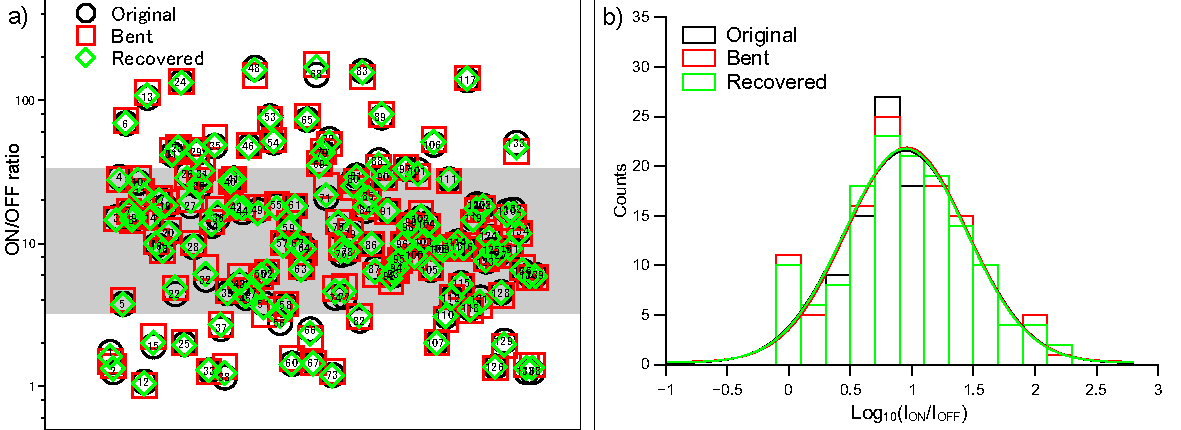
\includegraphics[width=\textwidth]{figures/figure6_3}
\caption[Statistical distribution of ON/OFF ratios]
{Statistical distribution of the measured ON/OFF (photocurrent/dark current) ratios for 139 bending/recovery experiments undertaken on individual CdS nanowires. (a) ON/OFF ratio scatter; a gray region, where the majority of cases were documented, is drawn as a guide to the eye. (b) Statistical analysis of the data in (a); the lines represent Gaussian fits to the 3 histograms.
\label{fig:6_3}}
\end{figure}

As shown in Figure \ref{fig:6_3}a, although the values vary from case to case, caused by probing-induced contact changes, the ON/OFF ratios are rather stable for each individual case. The statistical distribution of the ON/OFF values in Figure \ref{fig:6_3}b confirms this trend on a wider scale and also allows us to estimate an average value of around 10. The results of stable ON/OFF ratios were most common; however, some data showed deviations. The reason is the fact that our setup has limitations with respect to the number of electrodes employed. With only two electrodes, contact resistance becomes an important uncertainty.\cite{Hummelgard2011} The effects of this variable are however absorbed by our statistical analysis, where it is normally distributed. The independent nature of this variable with respect to the resistance of the nanowire itself allows their contributions to be separated, enabling us to observe the effects which are due to the intrinsic nature of our sample.

\begin{figure}  
\includegraphics[width=250pt]{figures/figure6_4}
\caption[Photocurrent spectroscopy of deformed CdS NW]
{Photocurrent spectroscopy measurements performed on a representative individual CdS nanowire. The spectra have been fitted with logistic decay functions (solid lines); the regions of the curves corresponding to the symmetry point of each function have been extrapolated (dashed lines) in order to determine the intersections with the horizontal asymptote (dotted line). Insets show a schematic of the bending experiment (lower-left) and a low-magnification TEM image of the selected nanowire in contact with the W probe (upper-right). The values of the applied elastic strain and experimental red shift are marked.
\label{fig:6_4}}
\end{figure}

In order to obtain additional information regarding the nanowires, we performed photocurrent spectroscopy and simultaneous HRTEM imaging. In Figure \ref{fig:6_4}, the photocurrent spectroscopy results are displayed before and during a bending process which introduces a 1.1\% elastic deformation. The nanowire photocurrent cut-off wavelength has a 7.3 nm red shift during bending: in the initial state, the edge wavelength was 521.8 nm; during bending, this value increased to 529.1 nm. Figure \ref{fig:6_s3} shows more examples which feature similar red-shifts for the cut-off wavelength. Overall, for 1.68\%, 0.75\%, 1.59\%, 1.21\% and 3.36\% strains, 1.2 nm, 5.4 nm, -0.6 nm, 0.7 nm and 5.5 nm shifts were recorded. We obtain an average value of $3.3\pm2.9$ nm; although there is some deviation in the data, it shows that the effect is not limited to individual cases. The cut-off value of the photocurrent spectra is related to band structure, which determines the near-band-edge emission (NBE) of the material. Our observations are consistent with previous work performed by measuring the cathodoluminescence of CdS nanowires inside SEM, where the authors observed red-shifted emission for the NBE peak under strain, which is an indication for a decrease in the bandgap value, in agreement with our data.\cite{Fu2011}

\begin{figure}  
\includegraphics[width=\textwidth]{figures/figure6_s3}
\caption[Photocurrent spectroscopy of deformed CdS NW]
{(a,b) Additional examples of photocurrent spectroscopy of individual CdS nanowires, in their initial and deformed states. Low magnification TEM images are shown in the insets for each case. Strain and red-shift values are marked on each of the plots. 
\label{fig:6_s3}}
\end{figure}


Evidence of the deformation effects which could have induced the valence band decrease can be found in the HRTEM images. Figure \ref{fig:6_5} shows an image of a typical bent CdS nanowire. The diameter was measured to be around 35.6 nm, and its bending radius was 1040.7 nm, leading to a strain of 2.42\%.  Figure \ref{fig:6_5}a is a high-resolution image taken from the area marked in Figure \ref{fig:6_5}b. The result of geometric phase analysis (GPA) performed on this high-resolution image is given in Figure \ref{fig:6_5}c; the data shows that the upper-left corner of the image, oriented towards the center of the nanowire, experiences more strain than the edge region of the nanowire, located in the lower-right corner of the same image. The same GPA analysis procedure allows us to infer the locations of several defects in this area, based on abrupt changes in the calculated phase. Other defects are also likely to be present, as indicated by several regions of different contrast which are visible in the same image. It should be noted that the present nanowires were deformed elastically, compared to the previous examples where they had undergone larger strains (>10\%).\cite{Wang2013}
It should be noted that the averaged results presented here cannot accurately describe any single selected nanowire in terms of performance. The nanowires vary in regards to their morphology and structural properties, even within the same batch. There is an inherent contradiction between the need to accurately control the properties of every nanowire and the high-yield production required for making multiple devices at an industrial scale. From a statistical point of view, within this variety of structures, the nanowires studied here share common features with respect to their photocurrent-to-dark current ratio behavior during the deformation cycles. This is particularly advantageous for devices manufactured from a large amount of nanowires. Indeed, successful examples of making flexible transparent electrodes,\cite{Liu2014a} flexible photodetectors,\cite{Xu2015b} flexible supercapacitor electrodes,\cite{Liu2014a} lithium-ion batteries,\cite{Wang2015} LED arrays,\cite{Wang2015a} solar cells,\cite{Zhang2012}. out of these structures have already been reported.\\

\begin{figure}  
\centering
\includegraphics[width=250pt]{figures/figure6_5}
\caption[Diffraction of NW under strain]
{(a,b) TEM images of the nanowire before/after bending on a TEM carbon grid using a standard double-tilt holder due to the electron beam irradiation of the supporting C segments. The insets show SAED patterns along the [001] direction from areas marked by red circles. Representative framed parts of the SAED patterns are zoomed-in in the lower-right parts of the panels.
\label{fig:6_5}}
\end{figure}

\section{Conclusion}
To summarize, we have successfully performed pioneering photocurrent measurements for elastically deformed CdS nanowires inside the HRTEM. Using in situ electrical probing and light illumination, we have characterized the electronic (dark, light-off) and optoelectronic (light-on) features of individual nanowires undergoing mechanical deformation. To make the data reliable in a view of future technological applications, a large variety of nanowires was tested, allowing for a statistical analysis of their properties. All nanostructures reveal very close photocurrent-to-dark current ratios (ON/OFF ratios) in original, bent and recovered states, with an average value of approximately 10. Photocurrent spectroscopy of several examples shows red shifts of the order of several nanometers for the photocurrent cut-off wavelength. These small shifts are likely caused by deformation, which induces variations in the band structure. By taking HRTEM images, non-uniformly distributed lattice defects were found after bending. Our experiments reveal a variety of bending-induced effects for individual nanowires, while showing that from a statistical point of view the nanowires display common features in their response to deformation, making them suitable for future flexible optoelectronic applications. 


%update: Dec 20 wrote more. 

\begin{savequote}[75mm] 
In three words I can sum up everything I've learned about life: it goes on.
\qauthor{Robert Frost} 
\end{savequote}

\chapter{Conclusions and Future Perspectives}

\newthought{In summary}, probing technique is applied to \emph{in situ} TEM.

\section{Conclusions}

\section{Future perspectives}
\subsection{Look back to histroy to see where we are}
Anthropologist belive that an evolution of mankind would be linked to the use of tools. \cite{lilley1948men} The acients made tools to handle things at meter scale, such as knife, wrench, scythe, sickle. Human civilization histroy is very much related to to development of tools. By updating tools, humankind are able to handle meter scale objects, and gradually a few scales different from our size. The advancement of tools development is directly determined by development of science and technology. 

From millions of years ago, humankind started to updating tools. During prehistroy (beore 3,000 BC) and ancient age (3,000 BC to 476 AC), more and more well made stone, bronze and iron made tools came out to serve human beings for daily use -- at a scale from centimeter to hundreds of meters. In paleolithic age, people are mainly making simple tools; while in neolithic age, people are experienced with applying tools to building constructions. The capability of human beings are still restricted withing 3 scales from ourselves. It is called {\em meter-scale age}. 
In medieval age (476 AC to 1492 AC), the development of classical optics, including the production of well-made lenses, laid the groundwork for microscopy -- the tool to reach microscale and astronomical scale. In modern age (1492 AC to 1789 AC), many revolutionary researches in optics and microscopy are associated and contributed to the fast development of physics, chemistry, biology and material science. It is called {\em micro-scale age}. 
During the last centry, development of partical physics, theory of relativity and quantum mechanics made it possible to see nanoscale world by electron microscopy and atomic force microscopy. It is called {\em nano-scale age}.

The important mark between each "scale age" is the invention of optical microscope and electron microscope, because the preliminary important thing to do with the scale is to see objects in that scale. The main activities at early stage of each "scale age" are development of the microscopy itself as well as observing and getting knowledge of the new world objects. The main activities at second stage of each "scale age" is the production of building blocks and applications in that scales. Only when people are very familiar with almost everything in that scale with daily used applications, then science advances might move to the next scale by the rising theories and exiting experiments. 


After developing precised mechanics, human are able to make fine mechanics to operate small objects. The gear was able to transfer larger movement into fine movements. The ratio could be improved by the development of advanced gearing. However, it is not until recent years that people are able to reach nanometer precision on mechanics when piezoelectric motor is available. \cite{} 

Clearly we are now in the cross road between first stage and second stage of the {\em nanoscale age}. 

\subsection{Nanoscale building blocks in future}
Although many researchers claim their nanomaterial samples are perfect and uniform, the quality is not as perfect to perform identical physical or chemical properties. In chapter 6, it is noticed that even the ratios of photo-to-dark current ratios in different states is more or less stable, the photo-to-current ratios of each nanowire is very differnt from each other. The scattered distribution of the ratios is caused by the uniform structural behavior and chemical composition. To use the nanowires in bundles is practical in some applications, while it is not practical to apply them in single nanowire devices as mass production. \\
It is expected that nanoscale building blocks can be really uniform at the nanoscale. What nanoscale building blocks to complicated nanoworld applications is the bricks to the architecture. When the synthesis of various nanoscale building blocks can be well controlled to reach identical morphology, surface and physical, chemical properties. 
Another problem is the understanding of many nanomaterials are not comprehensive. But if the materials are synthesized 

\subsection{Nanomanipulations via microscopy in future}
We are now in 2017, the age of nanotechnology, of gene eneineering, of information technology, artificial intellegence and many more. According to the history of tools, human beings are now quite new to nanometer scale. The tools we are using for the nano world are electron microscopy, atomic force microscopy, lithography, piezoelectric probing and other mechanical technologies. It is true that various nanostructures are successfully synthesized, designed electronic chips are in mass production, observations are performed at atomic resolution. However, lithography technology does not work for many other applications, microscopy has sampling limitations, mechanical technology is not mature yet to handle nanoscale building blocks easily. 

\begin{figure}  
\centering
\includegraphics[width=200pt]{figures/aifornanomanipulation}
\caption[AI for Nanomanipulation]
{The workflow for nanoscale manipulations by automation.
\label{fig:7_aiworkflow}}
\end{figure}

During my research for PhD degree, I successfully performed tousands of nanoscale operations mannually. Most processes are based on personal experience. If we are able to translate our experience into codes for machine, it is very possible that machines are able to perform the repeatable operations. In Figure \ref{fig:7_aiworkflow}, an example of automation of nanomanipulation is performed. In this workflow figure, the machine starts from sample loading, and then perform searching of qualified nanostructure targets, followed by automation of microscopy, second qualification check, autofocus and auto-alignment for high resolution imaging, third qualification check, determining location of probe and target sample, approaching and contacting probe to target, electron beam weldering, retract nanostructure target, and many other possible functions. 
Automation of nanoscale handling through SEM and AFM. \cite{Sergej Fatikow}

\subsection{Nanoscale energy storage in future}
Nanomaterials are superior in offering large surface to volume ratios, decent transport properties, variable physical parameters, and confinement effects resulting from the nanoscale dimensions, and have been extensively studied for energy-related applications such as solar cells, thermoelectrics, ion batteries, supercapacitors, and gas storage applications.\\
It is expected that the future energy storage are structurally designed down to nanoscale to fully ultilize the {\em 'plenty of room at the bottom'}. The volumetric capacity could be much higher while at the same time keep the battery stable and safe. 
(1) providing a large surface area to boost the electrochemical reaction or molecular adsorption occurring at the solid–liquid or solid–gas interfaces, (2) generating optical effects to improve optical absorption in solar cells, and (3) giving rise to high crystallinity and/or porous structures to facilitate the electron or ion transport and electrolyte diffusion, so as to ensure that the electrochemical process occurs with high efficiency. It is emphasized that, to further enhance the capability of nanostructured materials for energy conversion and storage, new mechanisms and structures are eagerly awaited. In addition to highlighting the obvious advantages of nanostructured materials, their limitations and challenges for the usage in solar cells, lithium ion batteries, supercapacitors, and hydrogen storage systems are also required for further research.\cite{qifengzhang2013csr}\\



%Disadvantages
%1.Nanoparticles may be more difficult to synthesize and their dimensions are difficult to control.
%2.High electrolyte/electrode surface area may lead to more significant side reactions with the electrolyte, and more complications while maintaining interparticle contacts.

%cite{Bruce2008}


\singlespacing\clearpage\bibliographystyle{siam}\clearpage
\addcontentsline{toc}{chapter}{References}\bibliography{references} \clearpage
\addcontentsline{toc}{chapter}{Publications and presentations}

\chapter*{Publications \& Presentations}
\section*{Journal articles}
\noindent
\subsection*{2016}
%\years{2016}
\noindent1. {\underline {Zhang C.}}, Cretu O., Kvashnin D., Kawamoto N., Mitome N., Wang X., Bando Y., Sorokin P., Golberg D. "Statistically analyzed photoresponse of elastically bent CdS nanowires probed by light-compatible {\em in situ} High-Resolution TEM". {\em Nano Letters} 16(10), 6008-6013(2016); \\[5pt]
\noindent2. \underline{Zhang C.}, Wang X., Liang Q., Liu X., Weng Q., Liu J., Yang Y., Dai Z., Ding K., Bando Y. Golberg D. "Amorphous phosphorus/nitrogen-doped graphene paper for ultrastable sodium-ion batteries". {\em Nano Letters} 16(3), 2054-2060(2016);\\[5pt]
\noindent3. Xue Y., Dai P., Jiang X., Wang X., \underline{Zhang C.}, Tang D., Weng Q., Wang X., Pakdel A., Tang C. Bando Y., Golberg D. "Template-free synthesis of boron nitride foam-like porous monoliths and their high-end applications in water purification". {\em Journal of Material Chemistry A} 4(4), 1469-1478(2016);\\[5pt]
\noindent4. Hou G., Cheng B., Cao Y., Yao M., Li B., \underline{Zhang C.}, Weng Q., Wang X., Bando Y., Golberg D., Yuan F. "Scalable production of 3D plum-pudding-like Si/C spheres: Towards practical application in Li-ion batteries". {\em Nano Energy} 24, 111-120(2016); \\

\subsection*{2015}
%\years{2015}
\noindent5. \underline{Zhang C.}, Xu Z., Tian W., Wang X., Bando Y., Fukata N., Golberg D. “{\em In situ} fabrication and optoelectronic analysis of axial CdS/p-Si nanowire heterojunctions in a high-resolution transmission electron microscope”.{\em Nanotechnology} 26, 154001-8(2015);\\[5pt]
\noindent6. Xu Z., \underline{Zhang C.}, Bando Y., Bai X.D., Golberg D. “Lateral piezopotential-gated field-effect transistor of ZnO nanowires”. {\em Nano Energy} 13, 233-239(2015);\\[5pt]
\noindent7. Weng Q.H., Wang X., \underline{Zhang C.}, Jiang X., Bando Y., Golberg D. “Supercapacitive energy storage performance of molybdenum disulfide nanosheets wrapped with micoporous carbons”. {\em Journal of Material Chemistry A} 3, 3097-3102(2015); \\[5pt]
\noindent8. Wang. X, Liu D., Weng Q., Liu J., Liang X., \underline{Zhang C.} "Cu/Li4Ti5O12 scaffold as superior anode for lithium-ion batteries". {\em NPG Asia Materials} 7, 171(2015); \\[5pt]
\noindent9. \underline{Zhang C.}, Xu Z., Golberg D. " Opto-mechano-electrical tripling in ZnO nanowires probed by photocurrent spectroscopy in a high-resolution transmission electron microscope ".  {\em Applied Physics Letters} 107, 091103(2015); \\[5pt] 
\noindent10. Xue Y., Jiang B., Bourgeois B., Dai P., Mitome M., \underline{Zhang C.}, Yamaguchi M., Matveev A., Tang C., Bando Y., Tsuchiya K., Golberg D. "Aluminum matrix composites reinforced with multi-walled boron nitride nanotubes fabricated by a high-pressure torsion technique". {\em Materials \& Design} 88, 451-460(2015);\\[5pt]
\noindent11. Weng Q., Ide Y., Wang X.B., Wang X., \underline{Zhang C.}, Jiang X., Xue Y., Dai P., Komaguchi K., Bando Y., Golberg D. "Design of BN porous sheets with richly exposed (002) plane edges and their application as TiO2 visible light sensitizer". {\em Nano Energy} 16, 19-27(2015);\\[5pt]
\noindent12. Dai P., Xue Y., Wang X., Weng Q., \underline{Zhang C.}, Jiang X., Tang D., Wang X., Kawamoto N., Ide Y., Mitome M., Golberg D., Bando Y. "Pollutant capturing SERS substrate: porous boron nitride microfibers with uniform silver nanoparticle decoration". {\em Nanoscale} 7(45), 18992-18997(2015);\\

\subsection*{2014}
%\years{2014}
\noindent13. \underline{Zhang C.}, Tian W., Xu Z., Liu J., Li S., Tang D.M., Cai X., Wang X.,Weng Q., Liao M., Kawamoto N., Bando Y., Golberg D. “Photosensing performance of branched CdS/ZnO heterostructures as revealed by in situ TEM and photodetector tests”, {\em Nanoscale} 6, 8084-8090(2014);\\[5pt]
\noindent14. Golberg D., \underline{Zhang C.}, Xu Z. “Cubic lattice nanosheets: Thickness-driven light emission”, {\em ACS Nano} 8(7), 6516-6519(2014);\\[5pt]
\noindent15. Tian W., \underline{Zhang C.}, Zhai T., Li S.L., Wang X., Liu J., Jie X., Liu D., Lioa M., Koide Y., Golberg D., Bando Y. "Flexible ultraviolet photodetectors with broad photoresponse based on branched ZnS-ZnO heterostructure nanofilms”. {\em Advanced Materials} 26, 3088-3093(2014);\\[5pt]
\noindent16. Wang X., Weng Q.H., Liu X., Wang X.B., Tang D.M., Tian W., \underline{Zhang C.}, Yi W., Liu D., Bando Y., Golberg D. “Atomistic origins of high rate capability and capacity of N-doped graphene for Lithium storage”. {\em Nano Letters} 14, 1164-1171(2014);\\[5pt]
\noindent17. Wang X., Chen Z., Liu D., Tian W., Wang Q., \underline{Zhang C.}, Liu J.W., Han L., Bando Y., Golberg D. “Tripled-yolked ZnO-CdS hollow spheres for semiconductor-sensitized solar cells”, {\em Particle \& Particle Systems Characterization} 31(7), 757-762(2014);\\

\subsection*{Previously}
%\years{2012-2013}
\noindent18. Tian W., \underline{Zhang C.}, Wang X., Golberg D., Bando Y. “Flexible SnO2 hollow nanosphere film based high-performance ultraviolet photodetector”. {\em Chemical Communications} 49(36), 3739-3741(2013);\\[5pt]
\noindent19. Tian W., \underline{Zhang C.}, Wang X., Golberg D., Bando Y. "Flexible ultraviolet photodetectors with broad photoresponse based on branched ZnS-ZnO heterostructure nanofilms”. {\em Advanced Materials} 26(19), 3088–3093(2013);\\[5pt] 
\noindent20. Tian W. Wang X., Zhi C., Zhai T., Liu D., Zhang C., Golberg D., Bando Y. "Ni (OH)2 nanosheet@ Fe2O3 nanowire hybrid composite arrays for high-performance supercapacitor electrodes". {\em Nano Energy} 2(5), 754-763(2013).\\[5pt]
\noindent21. \underline{Zhang C.}, Huang H., Liang B., Wang X.F., Lan X., Xiang Q., Liu B., Chen D. "Patterned growth of In2O3 spheres organized by radially-aligned In2O3 nanobelts". {\em Journal of Nanoengineering and Nanomanufacturing} 2(2), 166-170(2012);\\[5pt]
\noindent22. Wang X.F., Huang H., Liu B., Liang B., \underline{Zhang C.}, Ji Q., Chen D., Shen G. "Shape evolution and applications in water purification: the case of CVD-grown Zn2SiO4 straw-bundles". {\em Journal of Material Chemistry} 22(12), 5330-5335(2012).\\

\section*{Oral presentations}

%\years{2016}
\noindent1. {\em Nanowire deformations and axial junction constructions in tandem with photocurrent measurements inside a transmission electron microscope}, MRS Spring 2016, Phoenix, USA(2016);\\[15pt]
%\years{2014}

\noindent2. {\em Optoelectronic properties of nanostructured materials as revealed by laser-compatible in situ Transmission Electron Microscopy}, 23rd Australian Conference on Microscopy and Microanalysis, Adelaide, Australia(2014). 

\section*{Poster presentations}
%\years{2016}
\noindent1. {\em Amorphous P@Graphene paper for ultrastable sodium-ion batteries}, AsiaNano 2016, Sapporo, Japan(2016);\\[15pt]
%\years{2015}
\noindent2. {\em In situ fabrication and photocurrent analysis of axial CdS/p-Si nanowire junctions by high-resolution TEM}, Japanese Society of Microscopy Kanto-branch meeting, Tokyo, Japan(2015). 



%\vspace{1cm}
\vfill{}
%\hrulefill\chapter*{Colophon}


\begin{center}

For my latest information of publications, please visit \\\url{https://scholar.google.com/citations?user=_tirUeIAAAAJ&view_op=list_works&sortby=pubdate}

Should you have any questions, please feel free to contact me by e-mail
\\\href{mailto:zhang.chao@nims.go.jp}{\nolinkurl{zhang.chao@nims.go.jp}} (until March 2017)
\\\href{mailto:zcelysium@gmail.com}{\nolinkurl{zcelysium@gmail.com}} (after March 2017)
\\[10ex]\emph{This is the end of the dissertation. } 

\end{center}

\end{document}
